\documentclass[UTF8]{ctexart}
\usepackage{graphicx}
\title{记录我的生活(关于自己在学习小组二代目的打卡)}
\author{Junital}
\begin{document}
\date{}
\maketitle
\begin{figure}[ht]
    \centering
    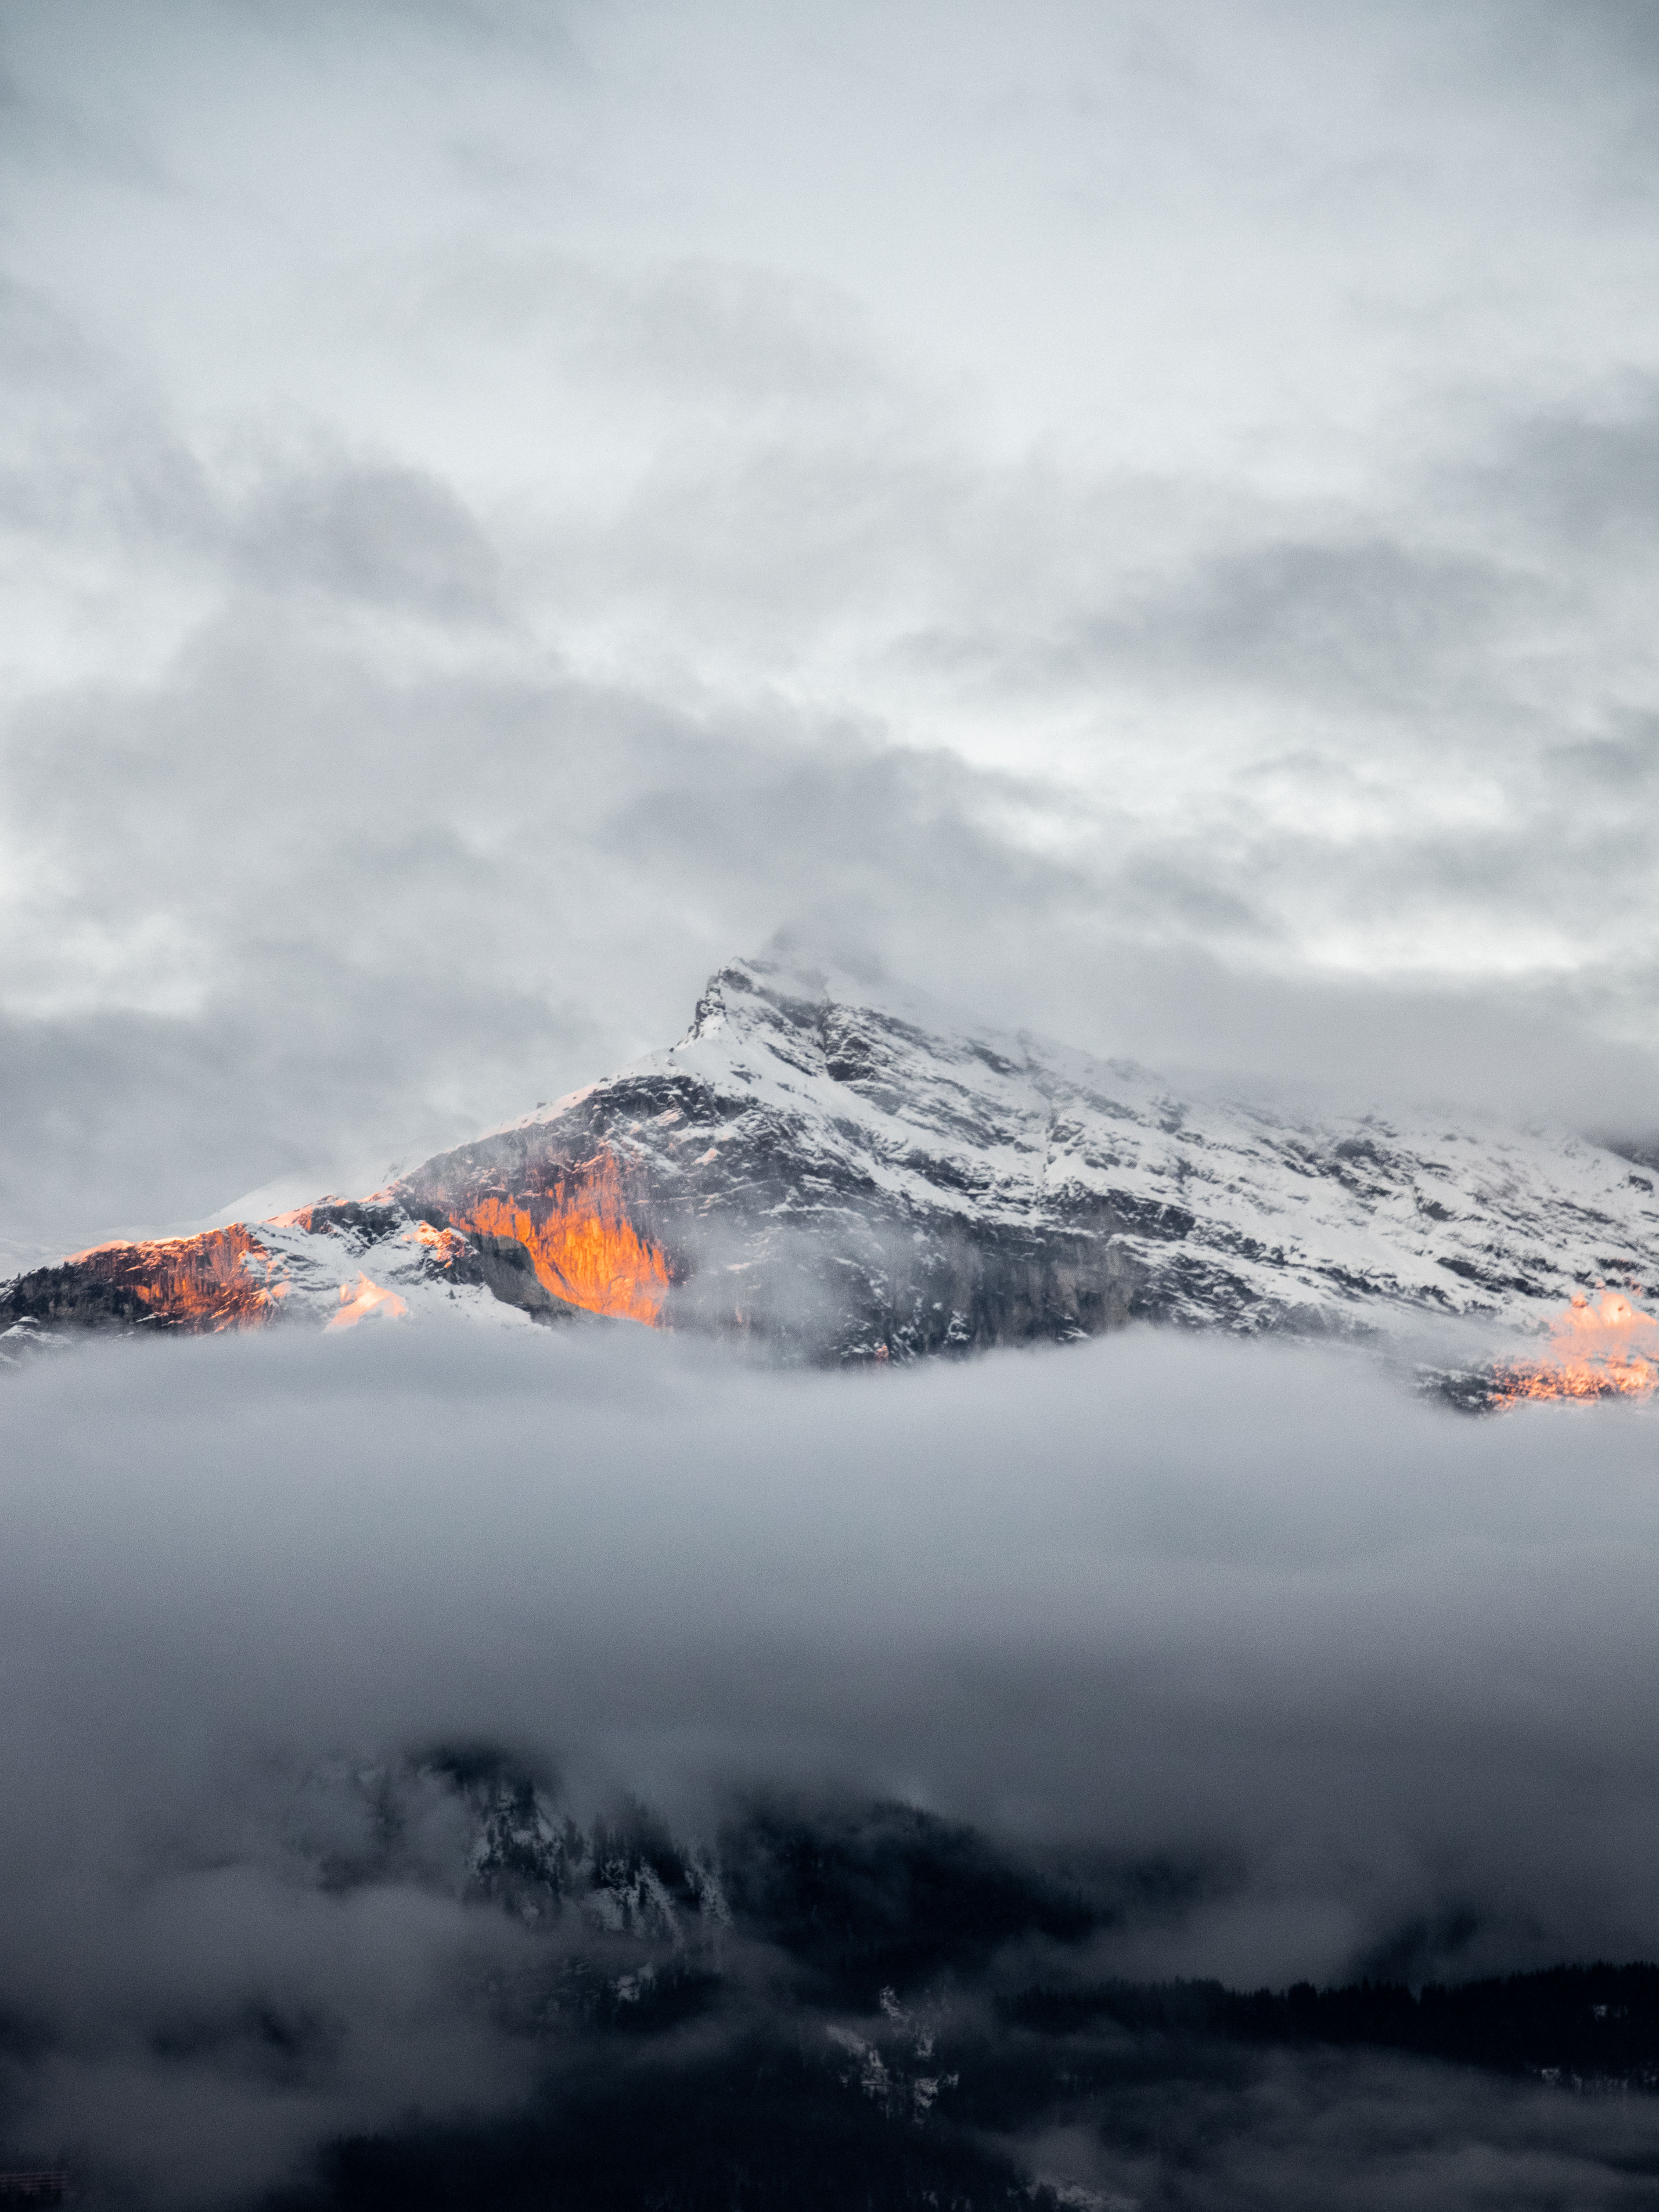
\includegraphics[width=0.65\textwidth]{./Figures/nicolas-savignat-wU5sBkxKtXs-unsplash.jpg}
    \nonumber
\end{figure}
\newpage
\section*{2022年11月}
\subsection*{11.13}
\begin{itemize}
    \item 完成计算机数学第二次作业
    \item 完成英语预习作业
    \item 提交机组第五次作业和大物作业
    \item 在\verb|VScode|上学习\LaTeX
    \item 和家人视频通话
    \item 离散复习(将群剩下的知识\verb|+|图论看完)
    \item 看电影《寻梦环游记》
    \item 背单词(\verb|10|生词\verb|+68|复习)
\end{itemize}
\subsection*{11.14}
\begin{itemize}
    \item 完成数据结构上机检查的任务
    \item 完成计算机数学第三次作业(没提交作业)
    \item 和\verb|FunMin|交流了一个半小时
    \item 完成物理模块总结
    \item 英语精听\verb|20min|
    \item 背英语单词(\verb|10|生词\verb|+|\verb|58|复习)
    \item \verb|P.S.| 今天离散未复习
\end{itemize}
\subsection*{11.15}
\begin{itemize}
    \item 完成数据结构头歌作业
    \item 英语精听\verb|20min|
    \item 背英语单词(\verb|10|生词\verb|+|\verb|58|复习)
    \item \verb|P.S.| 今天离散未复习
\end{itemize}
\subsection*{11.16}
\begin{itemize}
    \item 完成几何光学实验报告(未提交)
    \item 完成英语随堂测试
    \item 完成计数第四次作业
    \item 一套离散试卷
    \item 英语精听\verb|20min|
    \item 背英语单词(\verb|10|生词\verb|+|\verb|81|复习)
\end{itemize}
\subsection*{11.17}
\begin{itemize}
    \item 完成霍尔效应实验预习
    \item 英语精听\verb|20min|
    \item 背英语单词(\verb|10|生词\verb|+|\verb|62|复习)
    \item 离散数学环和域深入研究
\end{itemize}
\subsection*{11.18}
\begin{itemize}
    \item 完成物理第15次作业
    \item 完成马原第三次案例分析
    \item 听人工智能课两堂
    \item 英语精听\verb|20min|
    \item 比赛三题\verb|CF|
    \item 离散数学一套试卷
    \item 背英语单词(\verb|10|生词\verb|+|\verb|99|复习)
\end{itemize}
\subsection*{11.19}
\begin{itemize}
    \item 完成第六次机组作业
    \item 英语精听\verb|20min|
    \item 复习离散(复习所有知识点,温故知新,并检查校对之前做过的题目)
    \item 背英语单词(\verb|10|生词\verb|+|\verb|72|复习)
\end{itemize}
\subsection*{11.20(离散考试)}
\begin{itemize}
    \item 离散复习
    \item 看《末代皇帝》
    \item \verb|CF|三题打到下班
    \item 和家人视频通话
    \item 背英语单词(\verb|10|生词\verb|+|\verb|53|复习)
    \item 英语精听\verb|20min|
\end{itemize}
\subsection*{11.21}
\begin{itemize}
    \item 跑2400米(12min)
    \item 背英语单词(\verb|10|生词\verb|+|\verb|57|复习)
    \item 英语精听20min
    \item 共产党宣言(1030/3000)
    \item 英语预习作业完成
    \item 继续看《卡拉马佐夫兄弟》(暂时还没有感触的地方)
    \item 复习今天学到的知识
          \begin{itemize}
              \item 机数:Floor and ceiling,学会灵活使用在证明上
              \item 大物:相对论中的质量和因此推理出的质能方程,以及方程中动能、静能、动量的关系
          \end{itemize}
\end{itemize}
\subsection*{11.22}
\begin{itemize}
    \item 背英语单词(10生词\verb|+|63复习)
    \item 英语精听20min
    \item 《共产党宣言》感悟(2600\verb|/|3000)
    \item 跑2400米(10min 8s)
    \item 数据结构头歌作业完成一部分
    \item 跑完肚子好胀,不知道是不是喝了冷饮的原因QAQ
    \item 看《卡拉马佐夫兄弟》,对于神学有一点点感悟
    \item 复习今天学到的知识
          \begin{itemize}
              \item 机组:I\verb|/|O Technique的数据传送机制,Interrupt的运行原理
              \item 大英3:Rocket文章的行文思路,和文章细节的梳理
              \item 数据结构:树的复习总结和图的相关概念引入
              \item 马原:社会主义的历史发展
          \end{itemize}
\end{itemize}
\subsection*{11.23}
\begin{itemize}
    \item 背英语单词(10生词\verb|+|80复习)
    \item 英语精听20min
    \item 《共产党宣言》读后感(3500\verb|/|3000)
    \item 跑2400米(9min58s)
    \item 数据结构头歌作业完成(未提交)
    \item 物理作业完成(未提交)
    \item 看《卡拉马佐夫兄弟》
    \item 复习今天学到的知识
          \begin{itemize}
              \item 机数:$\left \lfloor \sqrt[3]{n}  \right \rfloor $ 和$spec(\alpha)$两种应用
              \item 大物:复习相对论基本知识,习题课
          \end{itemize}
\end{itemize}
\subsection*{11.24}
\begin{itemize}
    \item 背英语单词(10生词\verb|+|不知道复习了多少)
    \item 英语精听20min
    \item 英语外刊10min
    \item 跑1000米(4min30s)
    \item 把霍尔效应报告完成
    \item 给陈俊鑫老师写邮件
    \item 特色班登记
    \item 看《卡拉马佐夫兄弟》
    \item 复习今天学到的知识
          \begin{itemize}
              \item 数据结构:关于图的存储结构和遍历操作
              \item 马原:最终的共产主义
          \end{itemize}
\end{itemize}
\subsection*{11.25}
\centerline{一则故事}

我:坏了,没做核酸,我要死了。

班长:坏了,忘提醒做核酸,我要被骂了。

辅导员:坏了,要是学院怪在我身上,我就完了。

受伤的世界……
\begin{itemize}
    \item 背英语单词(10生词\verb|+|61复习)
    \item 英语精听20min
    \item 英语外刊10min
    \item 巨磁电阻报告预习
    \item 数据结构作业完成
    \item 看《卡拉马佐夫兄弟》
    \item 复习今天学到的知识
          \begin{itemize}
              \item 机组:Interrupt讲完加上DMA的相关知识
          \end{itemize}
\end{itemize}
\subsection*{11.26}
\begin{itemize}
    \item 背英语单词(10生词\verb|+|不知道复习了多少)
    \item 英语精听20min
    \item 英语外刊10min
    \item 跑步2400米(11min9s)
    \item VQA论文精读(终于读完了)
    \item 计算机数学作业完成(未提交)
    \item 考验功底的讲例会
    \item 和家人视频通话
    \item 看《卡拉马佐夫兄弟》
\end{itemize}
\subsection*{11.27}
\begin{itemize}
    \item 背英语单词(10生词\verb|+|不知道复习了多少)
    \item 英语外刊10min(直接蒙反而对太讽刺了)
    \item 英语四级模拟自测
    \item 数据结构代码
    \item 看《活着》
    \item 复习创思
    \item 看《卡拉马佐夫兄弟》
\end{itemize}
\subsection*{11.28}
\begin{itemize}
    \item 背英语单词(10生词\verb|+|65复习)
    \item 100俯卧撑
    \item 创思大作业完成(未提交)
    \item 英语作文初稿完成
    \item 看《卡拉马佐夫兄弟》
    \item 复习今天学到的知识
          \begin{itemize}
              \item 机数:利用floor and ceiling解决递归问题(高德纳数、Joseph问题)
              \item 大物:量子物理基本知识:热辐射、黑体辐射(三个公式)、光电效应
          \end{itemize}
\end{itemize}
\subsection*{11.29}
\begin{itemize}
    \item 背英语单词(10生词\verb|+|不知道复习了多少)
    \item 100俯卧撑
    \item 网球激情对打
    \item 看《卡拉马佐夫兄弟》
    \item 复习今天学到的知识
          \begin{itemize}
              \item 机组:关于CU的操作,指令具体的微操作
              \item 英语:1.test 2.presentation 3.essay-comment
              \item 数据结构:最小生成树(Prim+最小堆、Kruskal+并查集)
          \end{itemize}
\end{itemize}
\subsection*{11.30}
\begin{itemize}
    \item 背英语单词(10生词\verb|+|62复习)
    \item 100俯卧撑
    \item 数据结构并查集小代码
    \item 巨磁电阻报告完成(未提交)
    \item 复习马原第一章
    \item 看《卡拉马佐夫兄弟》
    \item 复习今天学到的知识
          \begin{itemize}
              \item 机数:将Joseph问题化为一般,利用MOD函数解决分组问题
              \item 大物:爱因斯坦的光量子理论和康普顿效应
          \end{itemize}
\end{itemize}
\section*{2022年12月}
\subsection*{12.1}
\begin{itemize}
    \item 背英语单词(10生词\verb|+|62复习)
    \item 100俯卧撑
    \item 数据结构Dijkstra、Floyd浅敲一下
    \item 头歌作业做完一半
    \item 大物MOOC静电场单元测试
    \item 人工智能视频刷了一章
    \item 大物模块总结写了四分之一
    \item 看《卡拉马佐夫兄弟》
    \item 复习今天学到的知识
          \begin{itemize}
              \item 数据结构:最短路径(单源:Dijkstra,点对:Floyd)
          \end{itemize}
\end{itemize}
\subsection*{12.2}
\begin{itemize}
    \item 背英语单词(10生词\verb|+|59复习)
    \item 100俯卧撑
    \item 人工智能视频刷了一章
    \item 大物模块总结还剩$\frac{1}{4}$
    \item 大物第17次作业
    \item 计算机数学作业完成
    \item 复习马原第二章
    \item 看《卡拉马佐夫兄弟》
    \item 听书《亲密关系》
    \item 复习今天学到的知识
          \begin{itemize}
              \item 机组:关于CU的硬件控制微操作的原理。
          \end{itemize}
\end{itemize}
\subsection*{12.3}
\begin{itemize}
    \item 背英语单词(10生词\verb|+|65复习)
    \item 100俯卧撑
    \item 人工智能视频刷了一章
    \item 大物第18次作业
    \item 大物MOOC恒定磁场单元测试
    \item 看《卡拉马佐夫兄弟》
    \item 大物模块总结完成,顺便复习了康普顿效应和静电场知识
    \item 马原第三章复习
\end{itemize}
\subsection*{12.4}
\begin{itemize}
    \item 背英语单词(10生词\verb|+|忘记复习了多少)
    \item 100俯卧撑
    \item 人工智能视频刷了一章
    \item 看《指环王1》
    \item 看《卡拉马佐夫兄弟》
    \item 大英作文修改并预习下一课文
    \item 英语听力仿真
    \item 马原第四章复习
\end{itemize}
\subsection*{12.5}
\begin{itemize}
    \item 早起第一天
    \item 背英语单词(10生词\verb|+|66复习)
    \item 100俯卧撑
    \item 重写入党申请书,誊抄3月份感想
    \item 今日计算机数学作业
    \item 复习马原第五章
    \item 看《卡拉马佐夫兄弟》
    \item 复习今天学到的知识
          \begin{itemize}
              \item 机数:Floor and ceiling的求和问题、二项式系数
              \item 大物:玻尔氢原子模型、德布罗意物质波
          \end{itemize}
\end{itemize}
\subsection*{12.6}
\begin{itemize}
    \item 早起第二天
    \item 背英语单词(10生词\verb|+|75复习)
    \item 100俯卧撑
    \item 写六月份感想(关于坚持)
    \item 复习马原第六章
    \item 头歌作业写完(未提交)
    \item 看《卡拉马佐夫兄弟》
    \item 复习今天学到的知识
          \begin{itemize}
              \item 机组:CU微指令讲完
              \item 英语:Cloud computing \& essay讲解
              \item 数据结构:关键路径和拓扑排序
          \end{itemize}
\end{itemize}
\subsection*{12.7}
\begin{itemize}
    \item 早起第三天
    \item 背英语单词(10生词\verb|+|81复习)
    \item 跑步2400米
    \item 写九月份感想(关于内卷)
    \item 复习马原第七章
    \item 检查大物作业和头歌作业
    \item 看《卡拉马佐夫兄弟》
    \item 复习今天学到的知识
          \begin{itemize}
              \item 机数:斯特林数与系数、概率
              \item 大物:不确定关系,薛定谔公式
          \end{itemize}
\end{itemize}
\subsection*{12.8}
\begin{itemize}
    \item 早起中断
    \item 背英语单词(10生词\verb|+|69复习)
    \item 物理第19次作业
    \item 写12月份感想(关于知行合一)
    \item 马原真题仿真
    \item 跑步2400米
    \item 四级阅读题练习
    \item 写大物小论文($\frac{1}{3}$)
    \item 没啥重要的了吧
    \item 看《卡拉马佐夫兄弟》
    \item 复习今天学到的知识
          \begin{itemize}
              \item 数据结构:关于静态排序(二分)和动态排序(二叉搜索树)
          \end{itemize}
\end{itemize}
\subsection*{12.9}
\begin{itemize}
    \item 早起第一天
    \item 背英语单词(10生词\verb|+|60复习)
    \item 根据大纲系统复习马原,查漏补缺,及时背诵
    \item 查Presentation资料
    \item 大物Mooc电磁感应
    \item 看《卡拉马佐夫兄弟》
    \item 复习今天学到的知识
          \begin{itemize}
              \item 机组:复习课(复习了第一、二章,还有很多没复习)
          \end{itemize}
\end{itemize}
\subsection*{12.10(四级考试)}
\begin{itemize}
    \item 早起第二天
    \item 背英语单词(10生词\verb|+|84复习)
    \item 大物小论文
    \item 马原大纲复习完,没有背
    \item Presentation初步制作
    \item 看《卡拉马佐夫兄弟》
    \item 和家人视频通话
\end{itemize}
\subsection*{12.11(马原考试)}
\begin{itemize}
    \item 早起第三天
    \item 复习马原
    \item 看《指环王2》没看完
    \item 看《卡拉马佐夫兄弟》
    \item 背英语单词(10生词\verb|+|不知道复习了多少)
\end{itemize}
\subsection*{12.12(润回家)}
\begin{itemize}
    \item 早起第四天
    \item 背英语单词(10生词\verb|+|不知道复习了多少)
    \item 补机数课和大物课
    \item 复习今天学到的知识
          \begin{itemize}
              \item 机数:抛硬币和方差问题
              \item 大物:量子几何分布
          \end{itemize}
\end{itemize}
\subsection*{12.13}
\begin{itemize}
    \item 早起第五天
    \item 背英语单词(10生词\verb|+|60复习)
    \item 机数作业
    \item 大物作业
    \item 数据结构头歌代码
    \item 复习今天学到的知识
    \item 准备英语pre
          \begin{itemize}
              \item 数据结构:插入排序和交换排序
          \end{itemize}
\end{itemize}
\subsection*{12.14}
\begin{itemize}
    \item 早起第六天
    \item 完成英语pre的ppt并试着录一次
    \item 完成自己的介绍ppt
    \item 完成人工智能视频
    \item 完成大物作业21
    \item 复习大物(电磁学)
    \item 背英语单词(10生词\verb|+|79复习)
\end{itemize}
\subsection*{12.15}
\begin{itemize}
    \item 早起第六天
    \item 看完《指环王2》
    \item 自己录了一遍pre
    \item 英语随堂作业做了一点点
    \item 大物复习了一点点
    \item 背英语单词(10生词\verb|+|66复习)
\end{itemize}
\subsection*{12.16(理性崩溃症病发)}
\begin{itemize}
    \item 早起中断
    \item 英语随堂作业做完
    \item 背英语单词(10生词\verb|+|71复习)
    \item 下午研究合桃派和复旦讲座
\end{itemize}
\subsection*{12.17}
\begin{itemize}
    \item 复习机组三章
    \item 看《卡拉马佐夫兄弟》
    \item 背英语单词(10生词\verb|+|68复习)
    \item 复旦讲座看完
    \item 特色班面试
    \item 数据结构MOOC与头歌完成
\end{itemize}
\subsection*{12.18}
\begin{itemize}
    \item 看《卡拉马佐夫兄弟》
    \item 跑步2400米
    \item 背英语单词(10生词\verb|+|67复习)
    \item 复习物理电磁学
    \item 看《指环王3》
\end{itemize}
\subsection*{12.19}
\begin{itemize}
    \item 跑步2400米
    \item 背英语单词(10生词\verb|+|79复习)
    \item 费曼物理复习完大物
    \item 将所有机组PPT看完
\end{itemize}
\subsection*{12.20}
\begin{itemize}
    \item 跑步2400米
    \item 背英语单词(10生词\verb|+|66复习)
    \item 补数据结构笔记,查漏补缺
    \item 计算机数学看了一下前三章
\end{itemize}
\subsection*{12.21}
\begin{itemize}
    \item 跑2400米
    \item 背英语单词(10生词\verb|+|66复习)
    \item 计算机数学剩下三章温习完
\end{itemize}
\subsection*{12.22}
\begin{itemize}
    \item 跑2400米
    \item 背英语单词(10生词\verb|+|68复习)
    \item 大物MOOC单元测试
\end{itemize}
\subsection*{12.23}
\begin{itemize}
    \item 跑2400米
    \item 背英语单词(10生词\verb|+|62复习)
    \item 大物MOOC期末测试
    \item 数据结构模拟卷
    \item 大物讨论题
\end{itemize}
\subsection*{12.24}
\begin{itemize}
    \item 跑2400米
    \item 背英语单词(10生词\verb|+|64复习)
    \item 数据结构讨论
    \item 计算机数学模拟卷
    \item 大物量子物理复习
\end{itemize}
\subsection*{12.25}
\begin{itemize}
    \item 跑2400米
    \item 背英语单词(10生词\verb|+|62复习)
    \item 大物除量子物理复习
    \item 复习机组
\end{itemize}
\subsection*{12.26(机组考试)}
\begin{itemize}
    \item 复习机组
\end{itemize}
\subsection*{12.27(机数考试)}
\begin{itemize}
    \item 复习机数
    \item 背英语单词
\end{itemize}
\subsection*{12.28(数据结构考试)}
\begin{itemize}
    \item 复习数据结构
\end{itemize}
\subsection*{12.29(大物考试)}
\begin{itemize}
    \item 复习大物
    \item 背英语单词
    \item 复习英语口试
\end{itemize}
\subsection*{12.30(英语口试)}
\begin{itemize}
    \item 复习英语口试
\end{itemize}
\subsection*{12.31}
\begin{itemize}
    \item 看《怪奇物语》第四季6集
    \item 看《古代文学常识》两章(天文、历法)
    \item 人工智能考试
    \item 背英语单词(10生词\verb|+|150复习)
    \item 12月总结
\end{itemize}
\section*{2023年1月}
\subsection*{1.1}
\begin{itemize}
    \item 看完《怪奇物语》第四季
    \item 看《模仿游戏》
    \item 看《古代文学常识》十章(车马、地理、官职、宫室、饮食、姓名、宗族、科举、礼俗、衣饰)
    \item 英语pre完结
    \item 背英语单词(10生词\verb|+|86复习)
\end{itemize}
\subsection*{1.2}
\begin{itemize}
    \item 看《古代文学常识》(什物)
    \item 日常代码4题
    \item 《我们为什么要睡觉》博客
    \item “如何辨别科学和伪科学”讲座
    \item 背英语单词(10生词\verb|+|52复习)
\end{itemize}
\subsection*{1.3}
\begin{itemize}
    \item 选课纠结中···
    \item 背英语单词
    \item 学了一点点计算机网络和操作系统
\end{itemize}
\subsection*{1.4}
\begin{itemize}
    \item 学习计算机网络一章
    \item Daily dictation
    \item 背英语单词
    \item 看《老友记》学英语,两集
    \item 选课确定了
\end{itemize}
\subsection*{1.5}
\begin{itemize}
    \item 计算机网络第一章学完
    \item Daily dictation
    \item 背英语单词
    \item 看《老友记》学英语,三集
    \item 看《寄生兽》看3集到第10集
    \item 看《操作系统》、《推荐系统》、《矩阵的力量》
    \item 看基于算法的个性化推荐影响讲座
    \item 和睿婷学姐商量华为ICT比赛
\end{itemize}
\subsection*{1.6}
\begin{itemize}
    \item 看《寄生兽》两集
    \item 看《老友记》学英语,两集
    \item Daily dictation
    \item 计算机网络 应用层Web方面知识
    \item 背英语单词
\end{itemize}
\subsection*{1.7}
\begin{itemize}
    \item 选体育课
    \item Daily dictation
    \item 背英语单词
    \item 看《牧马人》
    \item 当评优评委
    \item 观看实践直播
    \item 日常代码3题
\end{itemize}
\subsection*{1.8}
\begin{itemize}
    \item Daily dictation
    \item 背英语单词
    \item 看《寻妈记》5集
    \item 一周总结
    \item 日常代码3题
\end{itemize}
\subsection*{1.9}
\begin{itemize}
    \item Daily dictation
    \item 背英语单词
    \item 看《寻妈记》10集
    \item 代码2题
    \item 计算机网络SMTP篇
\end{itemize}
\subsection*{1.10}
\begin{itemize}
    \item Daily dictation
    \item 背英语单词
    \item 看《寻妈记》4集
    \item 计算机网络分布式
\end{itemize}
\subsection*{1.11}
\begin{itemize}
    \item 游玩天安门和国家博物馆
    \item 吃新疆菜(脆皮茄子很好吃)
    \item 游玩党史馆
    \item 吃火锅
\end{itemize}
\subsection*{1.12}
\begin{itemize}
    \item 看一下清华北大和国家图书馆
    \item 匆匆回家
\end{itemize}
\subsection*{1.13}
\begin{itemize}
    \item 买杯绿茶
    \item 背英语单词
    \item 看《寻妈记》10集
    \item Daily dictation
\end{itemize}
\subsection*{1.14}
\begin{itemize}
    \item 看《寻妈记》
    \item 背英语单词
    \item Daily dictation
    \item 看《性爱自修室》
    \item 量子位 知乎博主
\end{itemize}
\subsection*{1.15}
\begin{itemize}
    \item 看《寻妈记》
    \item 看《性爱自修室》
    \item 大创任务
    \item Daily dictation
    \item 知识管理\&时间管理
    \item 背英语单词
    \item 看《雷神:爱与雷霆》
\end{itemize}
\subsection*{1.16}
\begin{itemize}
    \item 看《寻妈记》
    \item 肝论文
    \item Daily dictation
    \item 意识流写作
    \item 计算机网络运输层
    \item 背英语单词
    \item 训练营比赛
    \item 学习Excel
\end{itemize}
\subsection*{1.17}
\begin{itemize}
    \item 看《寻妈记》
    \item 肝论文
    \item Daily dictation
    \item 意识流笔记
    \item 计算机网络运输层
    \item 背英语单词
    \item 动态规划学习
    \item 学习Excel
\end{itemize}
\subsection*{1.18}
\begin{itemize}
    \item 看《寻妈记》
    \item 肝论文
    \item Daily dictation
    \item 意识流笔记
    \item 计算机网络运输层结束
    \item 背英语单词
    \item 训练赛
    \item 学习Excel
\end{itemize}
\subsection*{1.19}
\begin{itemize}
    \item 看《寻妈记》
    \item 肝论文
    \item Daily dictation
    \item 意识流笔记
    \item 计算机网络网络层开始
    \item 背英语单词
    \item 动态规划学习
    \item 学习Excel
\end{itemize}
\subsection*{1.20}
\begin{itemize}
    \item 看《寻妈记》
    \item 肝论文
    \item Daily dictation
    \item 意识流笔记
    \item 计算机网络网络层开始
    \item 背英语单词
    \item 动态规划学习
    \item 学习Excel
\end{itemize}
\subsection*{1.21(大年夜)}
\begin{itemize}
    \item 论文粗稿提交
    \item 探寻心流秘境
    \item 拍照(主题二)
    \item 看望外公
    \item 垃圾桶之火
    \item Daily dictation
    \item 背英语单词
\end{itemize}
\subsection*{1.22(大年初一)}
\begin{itemize}
    \item 看《她》
    \item 玩游戏
    \item 研究TiddlyWiki
    \item 背英语单词
    \item Daily dictation
\end{itemize}
\subsection*{1.23}
\begin{itemize}
    \item 学习“动机理论”
    \item 计算机网络学习
    \item 动归代码作业
    \item 学习Excel
    \item Matlab调数据
    \item 背英语单词
    \item Daily dictation
\end{itemize}
\subsection*{1.24}
\begin{itemize}
    \item 计算机网络学习
    \item 动规代码作业写完
    \item 学习Excel
    \item 学习微信小程序开发
    \item 背英语单词
    \item 动机理论(二)
    \item Daily dictation
    \item 意识流笔记
\end{itemize}
\subsection*{1.25}
\begin{itemize}
    \item 计算机网络学习
    \item 线性动态规划学习
    \item 学习微信小程序开发
    \item 双元法入门(二)
    \item 动机理论(三)
    \item Daily dictation
    \item 背英语单词
    \item 意识流笔记\&小世界听播客
\end{itemize}
\subsection*{1.26}
\begin{itemize}
    \item 计算机网络学习
    \item 线性动态规划学习
    \item 学习微信小程序开发
    \item Daily dictation
    \item 背英语单词
    \item 整理笔记
\end{itemize}
\subsection*{1.27}
\begin{itemize}
    \item 计算机网络学习(ipad好用)
    \item 线性动态规划学习
    \item 学习微信小程序开发 右侧列表视图渲染
    \item 学习概率论
    \item 整理笔记
    \item Daily dictation
    \item 背英语单词
\end{itemize}
\subsection*{1.28}
\begin{itemize}
    \item 意识流笔记
    \item “最小阻力之路”
    \item 看望外公
    \item 在干爷爷处吃饭
    \item 背英语单词
    \item Daily dictation
\end{itemize}
\subsection*{1.29}
\begin{itemize}
    \item 意识流笔记
    \item 看《我不是药神》
    \item SuperMemo初体验
    \item 小程序 题库部分
    \item 背英语单词
    \item Daily dictation
\end{itemize}
\subsection*{1.30}
\begin{itemize}
    \item 意识流笔记
    \item 计算机网络学完
    \item 概率论学习
    \item 背英语单词
    \item 寒假训练4
    \item 叔叔家吃火锅
    \item 小程序框架完成
    \item Daily dictation
\end{itemize}
\subsection*{1.31}
\begin{itemize}
    \item 意识流笔记
    \item 操作系统学习
    \item 动态规划——子串
    \item 大创任务
    \item 小程序内容填充
    \item 背英语单词
    \item Daily dictation
    \item 美赛小会
\end{itemize}
\section*{2023年2月}
\subsection*{2.1}
\begin{itemize}
    \item 意识流笔记
    \item 操作系统学习
    \item 概率论学习(罗素悖论)
    \item 训练营比赛5
    \item 大创任务
    \item 小程序内容填充完毕
    \item 背英语单词
    \item Daily dictation
    \item Log-mode兴趣
\end{itemize}
\subsection*{2.2}
\begin{itemize}
    \item 意识流笔记
    \item 操作系统学习
    \item 概率论学习
    \item 线性动规作业
    \item 大创系统完成
    \item 小程序好难调
    \item 背英语单词
    \item Daily dictation
\end{itemize}
\subsection*{2.3}
\begin{itemize}
    \item 意识流笔记
    \item 操作系统学习
    \item 概率论学习
    \item 训练营比赛6
    \item 大创系统微调+模型代码找问题
    \item 小程序的内容部分没问题了
    \item 背英语单词
    \item Daily dictation
\end{itemize}
\subsection*{2.4}
\begin{itemize}
    \item 意识流笔记
    \item 看《洛奇》
    \item 和学长和老师交流大创一周总结
    \item 学习Log-mode
    \item 家庭会议\&理发
    \item 背英语单词
    \item Daily dictation
\end{itemize}
\subsection*{2.5}
\begin{itemize}
    \item 意识流写作
    \item 可视化学习
    \item 练习钢琴\&打篮球
    \item 可视化学习
    \item Johnny学——Obsidian降本提效
    \item 背英语单词
    \item Daily dictation
\end{itemize}
\subsection*{2.6}
\begin{itemize}
    \item 意识流写作
    \item 可视化学习
    \item 代码练习
    \item 学习操作系统
    \item 学习概率论
    \item 大创概率分布可视化
    \item 背英语单词
    \item Daily dictation
\end{itemize}
\subsection*{2.7}
\begin{itemize}
    \item 意识流写作
    \item 可视化学习
    \item 代码练习
    \item 学习操作系统
    \item 学习概率论
    \item 大创词频统计+异常检测照搬
    \item 背英语单词
    \item Daily dictation
\end{itemize}
\subsection*{2.8}
\begin{itemize}
    \item 意识流写作
    \item 数据库学习
    \item 代码练习
    \item 学习操作系统
    \item 学习概率论
    \item 大创异常检测调试,作者回复爬虫代码
    \item 背英语单词
    \item Daily dictation
\end{itemize}
\subsection*{2.9}
\begin{itemize}
    \item 意识流写作
    \item 数据库学习
    \item 代码练习
    \item 学习概率论
    \item 大创项目作者回复、综合分数
    \item 背英语单词
    \item Daily dictation
\end{itemize}
\subsection*{2.10}
\begin{itemize}
    \item 意识流写作
    \item 数据库学习
    \item 代码练习
    \item 学习概率论
    \item 大创异常检测模型没跑通
    \item 小程序收尾并发布
    \item Daily dictation
    \item 背英语单词
\end{itemize}
\subsection*{2.11}
\begin{itemize}
    \item 意识流写作
    \item 跟老师汇报一周工作
    \item 看《洛奇2》
    \item 学习Vim,顺便写几题
    \item 整理竞赛代码
    \item Zotero学习
    \item Daily dictation
    \item 背英语单词
\end{itemize}
\subsection*{2.12}
\begin{itemize}
    \item 意识流写作
    \item 看《寻妈记》
    \item 双元法学习
    \item 纯数学神经网络(未调试完)
    \item 小程序项目
    \item 背英语单词
    \item Daily dictation
\end{itemize}
\subsection*{2.13}
\begin{itemize}
    \item 意识流写作
    \item 数模流程图\&美赛论文模板
    \item 数据库学习
    \item 概率论学习
    \item 大创项目负面分数
    \item 纯数学神经网络
    \item 背英语单词
    \item Daily dictation
\end{itemize}
\subsection*{2.14}
\begin{itemize}
    \item 意识流写作
    \item 大创项目回复代码
    \item 软著手册
    \item 玩一下午(吴江)
    \item 代码练习
    \item 背英语单词
    \item Daily dictation
\end{itemize}
\subsection*{2.16}
\begin{itemize}
    \item 刷SuperMemo
    \item 整理行李
    \item 一下午返校
    \item 知乎大观园
    \item 收拾寝室
\end{itemize}
\subsection*{2.17}
\begin{itemize}
    \item 美赛比赛
    \item Daily dictation
    \item 刷SuperMemo
\end{itemize}
\subsection*{2.18}
\begin{itemize}
    \item 美赛比赛
    \item Daily dictation
    \item 刷SuperMemo
\end{itemize}
\subsection*{2.20}
\begin{itemize}
    \item 美赛比赛
    \item 计网上课
    \item 概率论上课
    \item 代码5h,值得记录
    \item Daily dictation
\end{itemize}
\subsection*{2.21}
\begin{itemize}
    \item 上课
    \item 概率论学习作业
    \item 上课音频查看
    \item 看ARM体系结构
    \item Daily dictation
    \item 整理ipad、待办、上课资源
\end{itemize}
\subsection*{2.22(特别2)}
\begin{itemize}
    \item 上课
    \item 整理音频
    \item 大创代码,词频特征
    \item 整理课程音频
    \item Daily dictation
    \item 计网作业
    \item 批判性阅读作业
\end{itemize}
\subsection*{2.23}
\begin{itemize}
    \item 上课
    \item Daily dictation
    \item 大创分数转换代码,尝试将评论作者参与度作为模型变量
\end{itemize}
\subsection*{2.24}
\begin{itemize}
    \item 上课
    \item Daily dictation
    \item 大创结果初见、服务器跑代码、跟老师汇报
    \item 概率论作业
    \item 计网作业
    \item 网球激情对打
\end{itemize}
\subsection*{2.25}
\begin{itemize}
    \item Daily dictation
    \item 网球激情对打
    \item 计网作业
    \item 和家人视频通话
    \item VDHL学习
    \item 网络编程
    \item 刷SuperMemo
\end{itemize}
\subsection*{2.26}
\begin{itemize}
    \item 刷SuperMemo
    \item 和家人视频通话
    \item MedVQA学习
    \item 代码练习
    \item Daily dictation
\end{itemize}
\subsection*{2.27}
\begin{itemize}
    \item 上课
    \item 计网音频
    \item 人脸识别python大项目
    \item 概率论课后习题
    \item 网球考试
    \item Daily dictation
\end{itemize}
\subsection*{2.28}
\begin{itemize}
    \item 上课
    \item 毛概音频
    \item VHDL CNN代码
    \item 概率论作业2
    \item 大创系统移植
    \item Daily dictation
    \item 刷SuperMemo
\end{itemize}
\section*{2023年3月}
\subsection*{3.1}
\begin{itemize}
    \item 上课
    \item 跟陈俊鑫老师聊天
    \item 大创系统增加内容
    \item Daily dictation
    \item 嵌入式报告
    \item 刷SuperMemo
\end{itemize}
\subsection*{3.2}
\begin{itemize}
    \item 上课
    \item 大创代码调试的不错
    \item Daily dictation
    \item 刷SuperMemo
    \item 写预习报告(嵌入式)
\end{itemize}
\subsection*{3.3}
\begin{itemize}
    \item 上课
    \item 跟老师开会
    \item Daily dictation
    \item 刷SuperMemo
    \item 大创模型提升+汇报工作
    \item 理发
    \item 班会
    \item 整理信息
\end{itemize}
\subsection*{3.4}
\begin{itemize}
    \item 看《素媛》
    \item 计网作业
    \item 散步
    \item VQA代码
    \item VIM学习
    \item 英语音频+讨论
    \item Daily dictation
\end{itemize}
\subsection*{3.5}
\begin{itemize}
    \item 计网作业
    \item VIM学习
    \item VQA代码
    \item 英语拟一个稿子
    \item 毛概音频
    \item 嵌入式代码
    \item 计网和操作系统音频
    \item Daily dictation
    \item 刷SuperMemo
\end{itemize}
\subsection*{3.6}
\begin{itemize}
    \item 上课
    \item 毛概看书
    \item 表情识别
    \item 大创论文完善
    \item Daily dictation
    \item 概率论作业写了一点
\end{itemize}
\subsection*{3.7}
\begin{itemize}
    \item 上课
    \item Daily dictation
    \item 大创论文完善
    \item VQA代码,读了论文
    \item 英语复习+对答案
\end{itemize}
\subsection*{3.8}
\begin{itemize}
    \item 上课
    \item Daily dictation
    \item 嵌入式报告
    \item 大创论文完善
    \item VQA代码,读了论文
    \item 毛概音频
\end{itemize}
\subsection*{3.9}
\begin{itemize}
    \item 上课
    \item Daily dictation
    \item 大创论文完善
\end{itemize}
\subsection*{3.10}
\begin{itemize}
    \item 上课
    \item 大创论文小稿提交
    \item Daily dictation
    \item VQA项目跑起来
    \item Linux环境搭建,跑C++代码
\end{itemize}
\subsection*{3.11}
\begin{itemize}
    \item 计算机网络作业
    \item Linux网络编程
    \item 确实该聊聊
    \item Daily dictation
    \item 看《爆裂鼓手》
    \item 玩玩树莓派
\end{itemize}
\subsection*{3.12}
\begin{itemize}
    \item 概率论作业
    \item 计算机网络作业
    \item 机器人琢磨
    \item 思想汇报
    \item 操作系统书再看
    \item 线段树
    \item Daily dictation
    \item 和家人视频通话
\end{itemize}
\subsection*{3.13}
\begin{itemize}
    \item 大创OpenReview的打分
    \item Daily dictation
    \item 上课
    \item 英语作业
    \item 思想汇报写完
    \item 志愿:整理图书
    \item 配置机器人环境
\end{itemize}
\subsection*{3.14}
\begin{itemize}
    \item 上课
    \item 嵌入式代码研究
    \item 英语作业写完
    \item 概率论作业
    \item 大创论文修改
    \item 刷SuperMemo
    \item Daily dictation
\end{itemize}
\subsection*{3.15}
\begin{itemize}
    \item 上课
    \item 嵌入式代码与报告
    \item 概率论作业
    \item 大创论文修改
    \item 刷SuperMemo
    \item Daily dictation
\end{itemize}
\subsection*{3.16}
\begin{itemize}
    \item 上课
    \item Daily dictation
    \item 写心得体会
    \item 大创论文完善
    \item 代码思路追寻
\end{itemize}
\subsection*{3.17}
\begin{itemize}
    \item 上课
    \item Daily dictation
    \item 计算机网络作业
    \item 农时宝创新点
    \item 大创项目论文完善
    \item 听操作系统音频
    \item VQA论文阅读
\end{itemize}
\subsection*{3.18}
\begin{itemize}
    \item 看《绿皮书》
    \item Daily dictation
    \item 录视频
    \item 选拔赛(勉勉强强)
    \item 完成论文讲解PPT
\end{itemize}
\subsection*{3.19}
\begin{itemize}
    \item 计算机网络作业
    \item 听讲座回放
    \item 操作系统练习
    \item 华为智能基座社团
    \item 完成选拔赛遗憾的题目
    \item 和家人视频通话
    \item 看计算机网络补充作业
\end{itemize}
\subsection*{3.20}
\begin{itemize}
    \item 上课
    \item Daily dictation
    \item 大创论文修改
    \item 概率论作业
    \item 嵌入式代码
\end{itemize}
\subsection*{3.21}
\begin{itemize}
    \item 上课
    \item 散步
    \item 洗澡
    \item 概率论作业
    \item 毛概看书
    \item Daily dictation
    \item 大创论文修改
\end{itemize}
\subsection*{3.22}
\begin{itemize}
    \item 上课
    \item Daily dictation
    \item 大创论文修改
    \item 概率论作业
    \item 毛概小班讨论主题确定、信息确认
    \item 嵌入式代码阅读
\end{itemize}
\subsection*{3.23}
\begin{itemize}
    \item 上课+实验
    \item Daily dictation
    \item 大创散点图绘制
    \item 小班讨论时间约定
\end{itemize}
\subsection*{3.24}
\begin{itemize}
    \item 上课
    \item Daily dictation
    \item 大创论文修改
    \item 概率论作业
    \item 见老师
    \item 毛概音频
\end{itemize}
\subsection*{3.25}
\begin{itemize}
    \item 计算机网络作业
    \item 概率论作业
    \item 开发区图书馆做志愿
    \item 看《铃芽之旅》
    \item 吃烤肉卷饼
    \item 写英语作业
    \item 跟ChatGPT从资本主义的消亡聊到小我和大我
\end{itemize}
\subsection*{3.26}
\begin{itemize}
    \item 计算机网络作业
    \item 操作系统实战
    \item 英语反思报告
    \item 海思嵌入式
    \item 毛概准备
    \item 跟家人通话
\end{itemize}
\subsection*{3.27}
\begin{itemize}
    \item 上课
    \item 洗澡
    \item Daily dictation
    \item 大创论文提交
    \item 嵌入式环境配置
    \item 概率论复习
    \item 写英语作业
\end{itemize}
\subsection*{3.28}
\begin{itemize}
    \item 上课
    \item Daily dictation
    \item 大创论文修改
    \item 嵌入式报告
    \item 英语报告修改
    \item 计算机网络音频
\end{itemize}
\subsection*{3.29}
\begin{itemize}
    \item 上课
    \item Daily dictation
    \item 大创代码任务
    \item 嵌入式代码准备
    \item 毛概音频
    \item 刷SuperMemo
\end{itemize}
\subsection*{3.30}
\begin{itemize}
    \item 上课
    \item Daily dictation
    \item 大创论文和实验修缮
\end{itemize}
\subsection*{3.31}
\begin{itemize}
    \item 上课
    \item Daily dictation
    \item 大创散点图任务
    \item 计算机网络作业
    \item 小班讨论的素材
    \item 嵌入式环境配置
    \item 英语翻译
    \item 嵌入式代码准备
\end{itemize}
\section*{2023年4月}
\subsection*{4.1}
\begin{itemize}
    \item 看《少年派的奇幻漂流》
    \item 计算机网络音频
    \item Daily dictation
    \item 述职报告想表达的内容
    \item 概率论上机
    \item 计算机网络作业
    \item 概率论大数定律、中心极限定理和t分布
    \item 和家人通话
\end{itemize}
\subsection*{4.2}
\begin{itemize}
    \item 计算机网络作业提交
    \item 述职报告思路
    \item 毛概音频
    \item Daily dictation
    \item Docker学习
    \item 概率论更详细的证明
    \item 英语Pre准备
    \item Keep一下
    \item 操作系统线程代码研究
    \item 概率论上机作业
    \item 嵌入式上机
    \item 概率论大数定律作业
\end{itemize}
\subsection*{4.3}
\begin{itemize}
    \item 上课
    \item Daily dictation
    \item 大创图片+实例准备
    \item 述职报告
    \item Docker初试
    \item 嵌入式大作业研究
    \item 华为云数据库
    \item 提交概率论第一次上机作业
    \item TED马斯克
    \item 畅想未来
    \item 修改PPT
\end{itemize}
\subsection*{4.4}
\begin{itemize}
    \item 上课
    \item Daily dictation
    \item 大创成果上交+实证研究
    \item TED马斯克2
    \item Docker小示例
    \item 查看毛概PPT
    \item 计算机网络音频
    \item 毛概交流
    \item 概率论音频
    \item 述职报告PPT制作
\end{itemize}
\subsection*{4.5}
\begin{itemize}
    \item Daily dictation
    \item 大创混合实验组数据
    \item 述职报告素材收集
    \item 制作操作系统入门
    \item 毛概小班讨论PPT最后改动
    \item 预测模型调试
    \item 述职报告制作
    \item 计算机网络前文回顾
\end{itemize}
\subsection*{4.6}
\begin{itemize}
    \item Daily dictation
    \item 上课
    \item 大创论文提交
    \item 述职报告最后收尾
    \item 操作系统输出
    \item 画简笔画
    \item 概率论作业提交
    \item Big picture
\end{itemize}
\subsection*{4.7}
\begin{itemize}
    \item 上课
    \item 述职报告
    \item Daily dictation
    \item 计算机网络作业
    \item 操作系统学习
    \item 拓扑学学习
\end{itemize}
\subsection*{4.8}
\begin{itemize}
    \item 操作系统音频
    \item Daily dictation
    \item 概率论上机
    \item 计算机网络作业
    \item 操作系统学习
    \item 英语文章与写作
    \item 跟妈妈通话
\end{itemize}
\subsection*{4.9}
\begin{itemize}
    \item 看《天使爱美丽》
    \item 计算机网络音频
    \item 树莓派学习
    \item 英语写作
    \item 学习拓扑学
    \item 操作系统建立
    \item 东北赛选拔赛
\end{itemize}
\subsection*{4.10}
\begin{itemize}
    \item Daily dictation
    \item 大创论文修改
    \item 上课
    \item 英语写作
    \item 概率论上机作业+下次作业
    \item 看毛概书
    \item 操作系统实操学习
    \item 嵌入式代码
\end{itemize}
\subsection*{4.11}
\begin{itemize}
    \item 上课
    \item Daily dictation
    \item 大创论文修改
    \item 树莓派学习
    \item 英语写作
    \item 概率论作业
    \item 英语Group Work
    \item 操作系统学习
\end{itemize}
\subsection*{4.12}
\begin{itemize}
    \item 上课
    \item Daily dictation
    \item 大创论文修改
    \item 树莓派学习
    \item 英语写作
    \item 概率论作业提交
    \item 科创PPT
    \item 毛概音频
\end{itemize}
\subsection*{4.13}
\begin{itemize}
    \item 上课
    \item Daily dictation
    \item 大创论文修改
    \item Daily translation
    \item 速通科创PPT制作
    \item Unit3Reflection
    \item 计算机网络音频
    \item 概率论音频+学习
\end{itemize}
\subsection*{4.14}
\begin{itemize}
    \item 上课
    \item Daily dictation
    \item 大创论文修改完毕
    \item Daily translation
    \item 计算机网络作业
    \item 嵌入式代码
\end{itemize}
\subsection*{4.15}
\begin{itemize}
    \item 看《何以为家》
    \item 华为音频
    \item 操作系统实战
    \item 嵌入式大作业最后冲刺失败
    \item 计算机网络作业提交
    \item 参观答辩
    \item Daily dictation
    \item 和家人视频通话
    \item Daily translation
\end{itemize}
\subsection*{4.16}
\begin{itemize}
    \item 制作完PPT
    \item 和刘扬河、左钧臣聊天
    \item 概率论作业
    \item CPC的CCCC热身赛
    \item 橙睿杯围观,拿到小礼品送人
    \item Daily dictation
    \item 操作系统互斥讨论
    \item Chat with ChatGPT
\end{itemize}
\subsection*{4.17}
\begin{itemize}
    \item 上课
    \item Daily dictation
    \item 大创论文
    \item 讲讲科创PPT
    \item 洗澡
    \item Daily translation
    \item 概率论作业10
    \item Reflection
    \item 机器人操作系统
\end{itemize}
\subsection*{4.18}
\begin{itemize}
    \item 上课
    \item Daily dictation
    \item 大创论文找文献
    \item Daily translation
    \item 概率论后半部分
    \item 形势与政策
    \item VQA可视化框架
\end{itemize}
\subsection*{4.19}
\begin{itemize}
    \item 上课
    \item Daily dictation
    \item 录视频+多模型VQA
    \item 大创论文参考文献
    \item Daily translation
    \item 概率论前半部分复习(kind of boring)
    \item 经典文献查看
    \item 计网音频+VQA打包失败
    \item 操作系统音频+课后题
\end{itemize}
\subsection*{4.20}
\begin{itemize}
    \item 上课
    \item Daily dictation
    \item 大创论文
    \item 英语作业
    \item Daily translation
    \item 概率论Chat复习
    \item 操作系统学习
    \item 计网音频
\end{itemize}
\subsection*{4.21}
\begin{itemize}
    \item 上课
    \item Daily dictation
    \item 大创论文
    \item 英语作业
    \item Daily translation
    \item 毛概音频
    \item 操作系统创建
    \item 用友音频
    \item 概率论复习
\end{itemize}
\subsection*{4.22}
\begin{itemize}
    \item Daily translation
    \item Daily dictation
    \item 数据音频$\times 2$
    \item 概率论练习复习
    \item 看《请以你的名字呼唤我》
    \item CCCC正式赛(发挥不太好
    \item B站库存
    \item 刷SuperMemo
\end{itemize}
\subsection*{4.23}
\begin{itemize}
    \item Daily dictation
    \item 上课
    \item 概率论2019年试卷
    \item 复习英语U4
\end{itemize}
\subsection*{4.24}
\begin{itemize}
    \item 上课
    \item Daily dictation
    \item 概率论复习(练习、检查、系统复习、Chat复习)
    \item Daily translation
    \item 学习系统讲座
    \item 毛概音频
    \item 经典文献阅读
    \item 英语复习
    \item 刷SuperMemo
\end{itemize}
\subsection*{4.25}
\begin{itemize}
    \item 上课
    \item 补机器人操作系统
    \item Daily dictation
    \item Daily translation
    \item 概率论复习(Chat复习、概念回顾、习题)
    \item 操作系统音频
    \item 英语复习+Group Work
\end{itemize}
\subsection*{4.26}
\begin{itemize}
    \item 上课
    \item 概率论考试
    \item 经典文献心得抄写
    \item Daily dictation
\end{itemize}
\subsection*{4.27}
\begin{itemize}
    \item 上课
    \item Daily dictation
    \item 去安盛游玩
\end{itemize}
\subsection*{4.28}
\begin{itemize}
    \item 上课
    \item 机器人操作系统
    \item Daily dictation
    \item Daily translation
    \item 毛概音频
    \item 英语作业
    \item 系统调试
    \item 学术预警小会
    \item 计网复习音频
\end{itemize}
\subsection*{4.29}
\begin{itemize}
    \item Daily translation
    \item 和家人视频通话
    \item 和电计同学交流系统
    \item 看《哈尔的移动城堡》
    \item 出去逛了一圈
    \item 刷SuperMemo
\end{itemize}
\subsection*{4.30}
\begin{itemize}
    \item Daily dictation
    \item 论文修改
    \item 操作系统同步练习
    \item 刷SuperMemo
    \item 计算机网络笔记整理
    \item Daily translation
    \item 合桃派直播,最小可行笔记系统
\end{itemize}
\section*{2023年5月}
\subsection*{5.1}
\begin{itemize}
    \item Daily dictation
    \item 论文修改
    \item 计算机网络第一二章
    \item 毛概音频
    \item 数据库音频
    \item 梳理操作系统任务
    \item Daily translation
\end{itemize}
\subsection*{5.2}
\begin{itemize}
    \item Daily dictation
    \item 论文修改
    \item 计算机网络第三四章
    \item 毛概音频
    \item 数据库音频
    \item 计算机网络有趣视频
    \item Daily translation
\end{itemize}
\subsection*{5.3}
\begin{itemize}
    \item Daily dictation
    \item 论文修改
    \item 操作系统音频
    \item 计算机网络有趣视频
    \item Daily translation
    \item 计算机深度搜索+专业术语
    \item 看《三国演义》
    \item 毛概音频
\end{itemize}
\subsection*{5.4}
\begin{itemize}
    \item 上课
    \item 计算机深度搜索
\end{itemize}
\subsection*{5.5}
\begin{itemize}
    \item 上课
    \item 计算机网络深度学习结束
    \item 计算机网络测验
    \item 刷SuperMemo+读道德经
\end{itemize}
\subsection*{5.6}
\begin{itemize}
    \item Daily Dictation
    \item 计算机网络检测后查漏补缺
    \item 看Pencil in Me
    \item 计算机网络最后冲刺
\end{itemize}
\subsection*{5.7}
\begin{itemize}
    \item 计算机网络最后的复习
    \item 看《蝙蝠侠:黑暗骑士》
    \item 跑步
    \item 计算机网络笔记电子化
\end{itemize}
\subsection*{5.8}
\begin{itemize}
    \item 上课
    \item 操作系统笔记整理
    \item 数据库笔记整理+正则表达式
    \item Daily dictation
    \item Daily translation
    \item Code cheat sheet
    \item 和家人视频通话
    \item 数据库上机
\end{itemize}
\subsection*{5.9}
\begin{itemize}
    \item 上课
    \item 操作系统笔记整理
    \item 数据库笔记整理
    \item Daily dictation
    \item 大创论文修改
    \item Daily translation
    \item Code cheat sheet制作
    \item 英语翻译
\end{itemize}
\subsection*{5.10}
\begin{itemize}
    \item 上课
    \item 嵌入式比赛学习
    \item Daily dictation
    \item 大创论文修改
\end{itemize}
\subsection*{5.11}
\begin{itemize}
    \item 上课
    \item Code Cheat Sheet
    \item 数据库笔记整理
    \item Daily Translation
    \item Daily Dictation
    \item 论文修改
    \item TED 演讲整理
\end{itemize}
\subsection*{5.12}
\begin{itemize}
    \item 上课
    \item TED ppt稿子改完
    \item Daily Translation
    \item Daily Dictation
    \item 操作系统笔记整理
    \item 大创论文修改
    \item 自学机器人操作系统
    \item 摄像头配置
\end{itemize}
\subsection*{5.13}
\begin{itemize}
    \item 到达哈尔滨
    \item 热身赛
    \item 博客更新
    \item 六级模拟
\end{itemize}
\subsection*{5.14}
\begin{itemize}
    \item 正式赛(被薄纱
    \item 回大连
    \item 写一些笔记
\end{itemize}
\subsection*{5.15}
\begin{itemize}
    \item 上课
    \item Dadily dictation
    \item 大创论文修改
    \item Daily translation
    \item 数据库笔记整理
    \item 毛概笔记整理
    \item 正则表达式学习
    \item 机器人操作系统作业
    \item 英语作业
    \item 嵌入式学习
\end{itemize}
\subsection*{5.16}
\begin{itemize}
    \item 上课
    \item Daily dictation
    \item 大创论文修改
    \item Daily translation
    \item 嵌入式学习
    \item PrePPT最后的构思
\end{itemize}
\subsection*{5.17}
\begin{itemize}
    \item 特色班开班仪式
    \item 研究摄像头开发板
\end{itemize}
\subsection*{5.18}
\begin{itemize}
    \item Daily Listening
    \item 大创论文模型调试
    \item 毛概整理
    \item 嵌入式比赛学习
    \item 研究摄像头开发板
\end{itemize}
\subsection*{5.19}
\begin{itemize}
    \item 英语听力
    \item 东北赛题目重想
    \item 大创论文
    \item 操作系统整理
    \item 清华科研项目开会
\end{itemize}
\subsection*{5.20}
\begin{itemize}
    \item 理发
    \item 毛概整理
    \item 嵌入式AI
    \item 和家人视频通话
    \item Daily translation
\end{itemize}
\subsection*{5.21}
\begin{itemize}
    \item 主校区嵌入式开会
    \item 英语背单词
    \item 解G题,好像找到了通解
    \item 毛概整理
\end{itemize}
\subsection*{5.22}
\begin{itemize}
    \item 英语单词
    \item 大创论文
    \item G题继续思考
    \item 毛概整理
    \item 英语作业
    \item 操作系统整理+sql练习
    \item 零碎碎片整理
\end{itemize}
\subsection*{5.23}
\begin{itemize}
    \item 英语听力
    \item 大创论文
    \item 毛概整理
    \item 操作系统整理
    \item SuperMemo和Logseq整理
    \item 笔记重新整理
\end{itemize}
\subsection*{5.24}
\begin{itemize}
    \item 上课
    \item 操作系统上机
\end{itemize}
\subsection*{5.25}
\begin{itemize}
    \item 上课
    \item 阅读AutoLM-GPT论文
    \item 开清华科研会议
    \item 毛概重点整理
    \item 操作系统报告
\end{itemize}
\subsection*{5.26}
\begin{itemize}
    \item 上课
    \item 研究ROS
    \item 操作系统实验报告
    \item 毛概系统整理
\end{itemize}
\subsection*{5.27}
\begin{itemize}
    \item 研究ROS
    \item 复习毛概
\end{itemize}
\subsection*{5.28}
\begin{itemize}
    \item 毛概最后复习
\end{itemize}
\subsection*{5.29}
\begin{itemize}
    \item 上课
    \item G题解出
    \item socket编程
    \item 数据库整理
    \item 操作系统上机准备了一点
    \item 海思服务器
\end{itemize}
\subsection*{5.30}
\begin{itemize}
    \item 操作系统oneAPI准备
    \item 操作系统整理
    \item 阅读论文
    \item 英语单词
    \item 英语听力
    \item ROS自动驾驶学习
\end{itemize}
\subsection*{5.31}
\begin{itemize}
    \item 论文阅读
    \item ROS自动驾驶学习
    \item 数据库作业
\end{itemize}
\section*{2023年6月}
\subsection*{6.1}
\begin{itemize}
    \item 论文阅读
    \item ROS学习
    \item 数据库作业
    \item 开会
    \item 选课
    \item 读论文
    \item 操作系统的Blog
\end{itemize}
\subsection*{6.2}
\begin{itemize}
    \item 看《蝙蝠侠:黑暗骑士崛起》
    \item 英语Reflection完成
    \item ROS没跑成功
\end{itemize}
\subsection*{6.3}
\begin{itemize}
    \item 数据库概念模型设计
    \item 数据库\&课堂笔记整理
    \item 体测
    \item 数据库线上测试
    \item ROS小车模型
    \item 劳动课感悟
\end{itemize}
\subsection*{6.4}
\begin{itemize}
    \item 自动驾驶继续推进,到物体识别框处。
    \item 英语段落选择
    \item 数据库网上测试
    \item 操作系统博客
\end{itemize}
\subsection*{6.5}
\begin{itemize}
    \item 自动驾驶继续推进
    \item 英语Reflection第二篇写完
    \item 局外人稿子确定
    \item 数据库网上测试
    \item 数据库、操作系统笔记整理
\end{itemize}
\subsection*{6.6}
\begin{itemize}
    \item 自动驾驶结束
    \item 整理小组报告内容
    \item 数据库线上测试
    \item 数据库+操作系统复习纲要
    \item 数据库作业
\end{itemize}
\subsection*{6.7}
\begin{itemize}
    \item 体育考试
    \item 自动驾驶报告温习
    \item 数据库线上测试
\end{itemize}
\subsection*{6.8}
\begin{itemize}
    \item 数据库线上测试
    \item 数据库大作业
    \item 操作系统复习
    \item 体育考试
    \item 上课
\end{itemize}
\subsection*{6.9}
\begin{itemize}
    \item 操作系统复习大纲更新
    \item 看操作系统书
    \item 看数据库书
    \item 英语六级阅读+单词背诵
    \item 数据库线上作业
    \item 数据库大作业
    \item 操作系统报告
\end{itemize}
\subsection*{6.10}
\begin{itemize}
    \item 操作系统自测
    \item 三刷肖申克
    \item 和家人通话
    \item 单词自测
    \item 操作系统大作业写完(未提交)
    \item 操作系统复习
    \item 整理操作系统ppt
\end{itemize}
\subsection*{6.11}
\begin{itemize}
    \item 数据库自测
    \item 单词自测
    \item 英语阅读练习
    \item 操作系统看PPT
    \item 操作系统报告
    \item 数据库概念部分
\end{itemize}
\subsection*{6.12}
\begin{itemize}
    \item 操作系统PPT刷完
    \item 英语单词自测
    \item 操作系统科普视频观看
    \item 数据库概念复习
    \item 讨论操作系统本质
\end{itemize}
\subsection*{6.13}
\begin{itemize}
    \item 操作系统最后复习
    \item 操作系统考试
    \item 略微复习了一下数据库
\end{itemize}
\subsection*{6.14}
\begin{itemize}
    \item 数据库的复习
    \item 数据库考试
    \item Manim尝鲜,就差中文的设置了
    \item 玩我的世界
    \item ROS报告
    \item 数据库笔记整理
\end{itemize}
\subsection*{6.15}
\begin{itemize}
    \item 复习英语六级和批判性阅读
    \item 今天上午和下午很不清醒,还好有YouTube和双仙保驾护航。
\end{itemize}
\subsection*{6.16}
\begin{itemize}
    \item 复习批判性阅读
    \item 考完休息了一晚上
\end{itemize}
\subsection*{6.17}
\begin{itemize}
    \item 备考六级
    \item 六级考试
    \item 和家人通话
\end{itemize}
\subsection*{6.19}
\begin{itemize}
    \item 写论文
    \item 嵌入式比赛服务器
    \item Codeforce训练
    \item 入党感想
\end{itemize}
\subsection*{6.20}
\begin{itemize}
    \item 嵌入式比赛服务器
    \item 写论文
    \item 活动计划书
    \item 知识管理论文阅读
\end{itemize}
\subsection*{6.21}
\begin{itemize}
    \item 嵌入式比赛
    \item 看奇异博士2
\end{itemize}
\subsection*{6.22}
\begin{itemize}
    \item 和蕊哥出去玩
\end{itemize}
\subsection*{6.23}
\begin{itemize}
    \item 论文
    \item 嵌入式比赛
    \item OS操作系统
\end{itemize}
\subsection*{6.24}
\begin{itemize}
    \item 嵌入式比赛
    \item RSIC-V操作系统
    \item ACM比赛
    \item Manim学习
\end{itemize}
\subsection*{6.25}
\begin{itemize}
    \item 嵌入式比赛
    \item ACM练习
    \item RISC-V操作系统
\end{itemize}
\subsection*{6.26}
\begin{itemize}
    \item ACM练习
    \item 看论文
\end{itemize}
\subsection*{6.27}
\begin{itemize}
    \item 看论文
    \item 嵌入式比赛学习
    \item 操作系统学习
    \item 论文代码优化
\end{itemize}
\subsection*{6.28}
\begin{itemize}
    \item 操作系统学习
    \item ACM刷题
    \item 看论文
\end{itemize}
\subsection*{6.29}
\begin{itemize}
    \item 讲论文
    \item 看论文
    \item 学习MindSpore
    \item 练习ACM
\end{itemize}
\subsection*{6.30}
\begin{itemize}
    \item 嵌入式比赛练习
    \item 论文实验部分完善
    \item 看书《三国》《认知驱动》
    \item 锻炼
    \item 科创比赛统计+随机写感想
\end{itemize}
\section*{2023年7月}
\subsection*{7.1}
\begin{itemize}
    \item 举办文艺活动
    \item 跑步 11:22秒 心率158 配速4'42
\end{itemize}
\subsection*{7.2}
\begin{itemize}
    \item 嵌入式比赛
    \item 跑步2400米
    \item 学习MindSpore
\end{itemize}
\subsection*{7.4}
\begin{itemize}
    \item 跑步2400米
    \item 论文修改
    \item 科创+活动总结
\end{itemize}
\subsection*{7.5}
\begin{itemize}
    \item 跑步2400米
    \item 嵌入式比赛
    \item 嵌入式操作系统学习
    \item 科创统计
    \item 论文修改
\end{itemize}
\subsection*{7.6}
\begin{itemize}
    \item 科创分享
    \item 跑步2400米
    \item 服务器训练
\end{itemize}
\subsection*{7.7}
\begin{itemize}
    \item 上课
    \item 嵌入式比赛
    \item 科创统计
    \item MindSpore模型运行
\end{itemize}
\subsection*{7.8}
\begin{itemize}
    \item 选课
    \item 社会实践——关向应纪念馆
    \item 数据集修改
\end{itemize}
\subsection*{7.9}
\begin{itemize}
    \item 看会电影
    \item 形势与政策
    \item 锻炼
\end{itemize}
\subsection*{7.10}
\begin{itemize}
    \item Python神经网络训练
    \item 嵌入式报告
    \item 嵌入式比赛最后报告指导
\end{itemize}
\subsection*{7.11}
\begin{itemize}
    \item Python报告+第四题可视化
    \item 电梯形式化设计思考
    \item 嵌入式比赛学习
\end{itemize}
\subsection*{7.12}
\begin{itemize}
    \item Python报告准备
\end{itemize}
\subsection*{7.13}
\begin{itemize}
    \item Python答辩
    \item 完成电梯形式化设计
    \item 嵌入式比赛进程推进
\end{itemize}
\subsection*{7.14}
\begin{itemize}
    \item 嵌入式比赛进程推进
    \item 录几个演示视频
\end{itemize}
\subsection*{7.15}
\begin{itemize}
    \item 睿抗比赛
    \item 嵌入式比赛操作部分收官
\end{itemize}
\subsection*{7.16}
\begin{itemize}
    \item 回家,放纵
\end{itemize}
\subsection*{7.17}
\begin{itemize}
    \item 嵌入式视频
    \item 操作系统报告
    \item 电梯代码实现
\end{itemize}
\subsection*{7.18}
\begin{itemize}
    \item 嵌入式比赛报告
    \item 嵌入式形式化设计报告
\end{itemize}
\subsection*{7.19}
\begin{itemize}
    \item 嵌入式比赛报告
    \item 形式化设计报告
\end{itemize}
\subsection*{7.23}
\begin{itemize}
    \item 软工学习
    \item 录视频
\end{itemize}
\subsection*{7.24}
\begin{itemize}
    \item 编译原理学习
    \item 嵌入式复赛准备
    \item ACM比赛
\end{itemize}
\subsection*{7.25}
\begin{itemize}
    \item 软工学习
    \item 修改论文
\end{itemize}
\subsection*{7.26}
\begin{itemize}
    \item 游玩北京
\end{itemize}
\subsection*{7.27}
\begin{itemize}
    \item 游玩北京
\end{itemize}
\subsection*{7.28}
\begin{itemize}
    \item 准备比赛
\end{itemize}
\subsection*{7.29}
\begin{itemize}
    \item 开始比赛
\end{itemize}
\subsection*{7.30}
\begin{itemize}
    \item 学习钢琴
    \item 看论文
    \item 解题(直角三棱锥)
\end{itemize}
\subsection*{7.31}
\begin{itemize}
    \item 看论文
    \item 学习胶囊网络
\end{itemize}

\section*{2023年8月}
\subsection*{8.1}
\begin{itemize}
    \item 看论文
    \item 学习软工
    \item 学习编译原理
\end{itemize}
\subsection*{8.2}
\begin{itemize}
    \item 看论文
\end{itemize}
\subsection*{8.3}
\begin{itemize}
    \item 看论文
\end{itemize}
\subsection*{8.4}
\begin{itemize}
    \item 摆烂
\end{itemize}
\subsection*{8.5}
\begin{itemize}
    \item 吃饭+摆烂
\end{itemize}
\subsection*{8.6}
\begin{itemize}
    \item 算法学习
    \item 驾照学习
    \item 看书《三国》
    \item 学习Manim
\end{itemize}
\subsection*{8.7}
\begin{itemize}
    \item 驾照学习
    \item 看书《三国》
    \item 算法学习
    \item 编译原理学习
    \item 软工学习
\end{itemize}
\subsection*{8.8}
\begin{itemize}
    \item 驾照学习
\end{itemize}
\subsection*{8.9}
\begin{itemize}
    \item 驾照学习
\end{itemize}
\subsection*{8.10}
\begin{itemize}
    \item 考驾照
    \item 献血
\end{itemize}
\subsection*{8.11}
\begin{itemize}
    \item 编译原理 + 软工学习
    \item 代码练习
    \item manim学习
\end{itemize}
\subsection*{8.12}
\begin{itemize}
    \item 代码练习
    \item 看看Stable Diffusion
\end{itemize}
\subsection*{8.13}
\begin{itemize}
    \item 代码练习
\end{itemize}
\subsection*{8.14}
\begin{itemize}
    \item 编译原理 + 软工学习
    \item 代码练习
    \item git练习
\end{itemize}
\subsection*{8.15}
\begin{itemize}
    \item 代码练习
    \item git练习
\end{itemize}
\subsection*{8.16}
\begin{itemize}
    \item 上午休息
    \item 下午和晚上也休息
\end{itemize}
\subsection*{8.17}
\begin{itemize}
    \item 休息
\end{itemize}
\subsection*{8.18}
\begin{itemize}
    \item 休息 + 比赛
    \item 正则表达式软件制作
\end{itemize}
\subsection*{8.19}
\begin{itemize}
    \item 休息
    \item SuperMemo视频观看
    \item Biomes开始玩玩
\end{itemize}
\subsection*{8.20}
\begin{itemize}
    \item WSL使用终端代理
    \item Biomes玩玩
    \item 学习编译原理
\end{itemize}
\subsection*{8.21}
\begin{itemize}
    \item 学习编译原理
\end{itemize}
\subsection*{8.22}
\begin{itemize}
    \item 正则表达式小软件终端版
    \item 学习编译原理(加油!
\end{itemize}
\subsection*{8.23}
\begin{itemize}
    \item 正则表达式终端版完成
    \item 学习编译原理(冲冲冲!!!
\end{itemize}
\subsection*{8.24}
\begin{itemize}
    \item 到外婆家玩
    \item 球球大作战达到大师级别
    \item 编译原理学完啦!!
\end{itemize}
\subsection*{8.25}
\begin{itemize}
    \item 准备开学
    \item 刷Logseq的卡片
\end{itemize}
\subsection*{8.26}
\begin{itemize}
    \item 飞机上看《三国》
    \item 前往大连
    \item 收拾宿舍
\end{itemize}
\subsection*{8.27}
\begin{itemize}
    \item AAAML环境 + ACM学习
    \item Modify README
    \item MCAN源码查看
    \item Prompt工程学习
\end{itemize}
\subsection*{8.28}
\begin{itemize}
    \item 上课
    \item 班内评选
    \item 奖学金查看
    \item 实践论文完成
\end{itemize}
\subsection*{8.29}
\begin{itemize}
    \item 上课
    \item ACM学习
    \item 奖学金细则
    \item 整理宿舍
\end{itemize}
\subsection*{8.30}
\begin{itemize}
    \item 上课
    \item 整理宿舍
    \item 吃水果
    \item ACM
    \item 背单词
    \item 补之前的课
\end{itemize}
\subsection*{8.31}
\begin{itemize}
    \item 上课
    \item 网络实验预习报告
    \item 吃水果
\end{itemize}
\section*{2023年9月}
\subsection*{9.1}
\begin{itemize}
    \item 上课
    \item 华为招聘会
    \item 党的思想报告
    \item 高级统计方法作业
    \item 奖学金了解
\end{itemize}
\subsection*{9.2}
\begin{itemize}
    \item 高级统计方法作业
    \item 《当幸福来敲门》
    \item 制作视频和信
    \item 软件工程录音
    \item 健身房
    \item 牛客 + 背单词
\end{itemize}
\subsection*{9.3}
\begin{itemize}
    \item 上课
    \item Prompt工程
    \item 背单词
    \item 实验报告
    \item SWEBOK完成
    \item MindSporeMCAN搭建环境
    \item 高级统计方法学习
\end{itemize}
\subsection*{9.4}
\begin{itemize}
    \item 上课
    \item 习概音频
    \item MCAN任务第一部分完成
    \item 高级统计方法作业
    \item 奖学金提交
\end{itemize}
\subsection*{9.5}
\begin{itemize}
    \item 上课
    \item 背单词
    \item Github整理
\end{itemize}
\subsection*{9.6}
\begin{itemize}
    \item 上课
    \item 背单词
    \item Github项目
    \item 习概音频
    \item 学习UI
\end{itemize}
\subsection*{9.7}
\begin{itemize}
    \item 上课
    \item 背单词
    \item Github项目
    \item 整理编译原理
    \item 阅读Image Stitching论文
\end{itemize}
\subsection*{9.8}
\begin{itemize}
    \item 上课
    \item 背单词
    \item MindSpore继续完成作业
    \item 编译技术作业
    \item 阅读论文
\end{itemize}
\subsection*{9.9}
\begin{itemize}
    \item 看《烈日灼心》
    \item 整理
    \item 剪视频
    \item MindSporeMCAN
    \item 背单词 + 视频听力
    \item 高统作业
\end{itemize}
\subsection*{9.10}
\begin{itemize}
    \item 背单词
    \item 上课
    \item 实验报告完成
    \item 整理
\end{itemize}
\subsection*{9.11}
\begin{itemize}
    \item 一整天上课
\end{itemize}
\subsection*{9.12}
\begin{itemize}
    \item 上课
    \item 整理奖学金
\end{itemize}
\subsection*{9.13}
\begin{itemize}
    \item 上课
    \item 背单词
    \item MindSporeMCAN
    \item 讨论实践选题
    \item 高统作业
    \item 把之前不懂的都整理了一下
\end{itemize}
\subsection*{9.14}
\begin{itemize}
    \item 上课
    \item 背单词
\end{itemize}
\subsection*{9.15}
\begin{itemize}
    \item 上课
    \item 背单词
    \item 实验报告完成
    \item 编译原理作业
\end{itemize}
\subsection*{9.16}
\begin{itemize}
    \item 看《疯狂动物城》
    \item 小班讨论选题确定
    \item 做视频、写信
    \item 高统作业、软工作业各一半
\end{itemize}
\subsection*{9.17}
\begin{itemize}
    \item 上课
    \item 背单词
    \item 高统上机
    \item 网综实验报告
\end{itemize}
\subsection*{9.18}
\begin{itemize}
    \item 上课
    \item 背单词
    \item 高统预习
    \item H3C模拟器
    \item 找视频素材
\end{itemize}
\subsection*{9.19}
\begin{itemize}
    \item 上课
    \item 背单词
    \item 习思想音频
    \item 报销
\end{itemize}
\subsection*{9.20}
\begin{itemize}
    \item 上课
    \item 背单词
    \item 高统补充
    \item 预习高统
    \item 拍摄
\end{itemize}
\subsection*{9.21}
\begin{itemize}
    \item 上课
    \item 背单词
    \item 报名
\end{itemize}
\subsection*{9.22}
\begin{itemize}
    \item 上课
    \item 背单词
    \item 可行性报告
    \item ACM
    \item 编译原理
    \item 软件工程笔记
    \item Prompt工程
\end{itemize}
\subsection*{9.23}
\begin{itemize}
    \item 背单词
    \item ACM
    \item 大创中期准备
    \item Prompt工程
    \item 软件工程作业
    \item 软件工程笔记
    \item 看《美国精神病人》
    \item 指导一下视频
    \item 网综实验报告
\end{itemize}
\subsection*{9.24}
\begin{itemize}
    \item 背单词
    \item 视频字幕
    \item 网综实验报告
    \item 预习高统
    \item 立项申报书
    \item 高统作业
    \item 发言稿
\end{itemize}
\subsection*{9.25}
\begin{itemize}
    \item 背单词
    \item 上课
    \item 高统作业
    \item 中期成果准备
    \item 网综模拟器
    \item Tarjan
\end{itemize}
\subsection*{9.26}
\begin{itemize}
    \item 背单词
    \item 上课
    \item 博弈树解决
\end{itemize}
\subsection*{9.27}
\begin{itemize}
    \item 上课
    \item 背单词
    \item 晒被子
    \item ACM
    \item 高统整理
    \item 中期成果准备
\end{itemize}
\subsection*{9.28}
\begin{itemize}
    \item 上课
    \item 背单词
    \item 分发奖品
\end{itemize}
\subsection*{9.29}
\begin{itemize}
    \item 背单词
    \item 习概音频
    \item ACM
    \item 网综报告
    \item 3D打印
    \item 图像拼接论文
    \item Prompt工程
    \item 中期成果、框架
    \item 赏月、跑步
\end{itemize}
\subsection*{9.30}
\begin{itemize}
    \item 背单词
    \item 剪视频 + 写信
    \item ACM
    \item Prompt工程
    \item 改革开放史
    \item 设计模式
    \item 看《无敌破坏王》
\end{itemize}
\section*{2023年10月}
\subsection*{10.1}
\begin{itemize}
    \item 背单词
    \item ACM
    \item 网综报告
    \item 习概音频
    \item 设计模式作业
    \item Prompt工程
    \item 软件工程音频
\end{itemize}
\subsection*{10.2}
\begin{itemize}
    \item 背单词
    \item ACM
    \item 网综报告
    \item 改革开放史音频
    \item Prompt工程
    \item 编译原理作业
    \item 论文阅读
\end{itemize}
\subsection*{10.3}
\begin{itemize}
    \item 背单词
    \item 网综实验
    \item 中期成果报告
    \item 思想实践立项
    \item ACM学习
    \item Prompt工程
    \item 跑步2400米
\end{itemize}
\subsection*{10.4}
\begin{itemize}
    \item 背单词
    \item 网综实验
    \item ACM学习
    \item RepaLLM
\end{itemize}

\subsection*{10.5}
\begin{itemize}
    \item 背单词
    \item 网综实验报告
    \item ACM学习
    \item 高统学习
    \item 编译原理上机
\end{itemize}
\subsection*{10.6}
\begin{itemize}
    \item 背单词
    \item 网综实验报告
    \item ACM学习
    \item 高统作业
    \item 软工学习
    \item 软工作业
    \item 理论课实践立项
\end{itemize}
\subsection*{10.7}
\begin{itemize}
    \item 理论课实践立项完成
    \item 上课
    \item 背单词
    \item RepaLLM继续推进
\end{itemize}

\subsection*{10.8}
\begin{itemize}
    \item 上课
    \item Paper Reading
    \item 背单词
    \item 高统上机
\end{itemize}

\subsection*{10.9}
\begin{itemize}
    \item 上课
    \item Paper Reading代码
    \item 背单词
    \item 国家奖学金申请
    \item 设计模式作业
\end{itemize}

\subsection*{10.10}
\begin{itemize}
    \item 上课
    \item 软件工程作业
    \item 背单词
    \item 奖学金准备
\end{itemize}

\subsection*{10.11}
\begin{itemize}
    \item 上课
    \item 背单词
    \item 准备答辩
    \item 高统作业提交
\end{itemize}

\subsection*{10.12}
\begin{itemize}
    \item 上课
    \item 背单词
    \item 准备答辩
    \item 正式答辩
    \item 软工作业
\end{itemize}

\subsection*{10.13}
\begin{itemize}
    \item 上课
    \item 背单词
    \item 剪视频
    \item 看《叫我第一名》
\end{itemize}

\subsection*{10.14}
\begin{itemize}
    \item 背单词
    \item ACM学习
    \item 编译原理作业
    \item 网综实验报告
    \item 习思想学习
    \item 写信
\end{itemize}

\subsection*{10.15}
\begin{itemize}
    \item 背单词
    \item 高统上机
    \item 网综实验报告
    \item 习思想学习
    \item 网综理论复习
\end{itemize}

\subsection*{10.16}
\begin{itemize}
    \item 背单词
    \item 高统上机
    \item 生日祝福
    \item 网综理论复习
\end{itemize}

\subsection*{10.17}
\begin{itemize}
    \item 背单词
    \item 复习网综实验
\end{itemize}

\subsection*{10.18}
\begin{itemize}
    \item 背单词
    \item 复习高统
    \item 高统应用题
    \item 写软工作业
    \item ACM学习
    \item 3D打印
\end{itemize}
\subsection*{10.19}
\begin{itemize}
    \item 高统作业
    \item 背单词
    \item 软工作业
\end{itemize}

\subsection*{10.20}
\begin{itemize}
    \item 高统作业
    \item 背单词
    \item 做PPT
\end{itemize}

\subsection*{10.21}
\begin{itemize}
    \item 背单词
    \item 设计模式PPT
    \item 做视频、写信
    \item 网综代码整理
    \item 看《三傻大闹宝莱坞》
\end{itemize}

\subsection*{10.22}
\begin{itemize}
    \item 背单词
    \item 网综报告
    \item 网综代码练习
    \item RepaLLM
    \item 编译原理作业
    \item 高统上机
\end{itemize}

\subsection*{10.23}
\begin{itemize}
    \item 背单词
    \item 网综代码练习
    \item 高统整理
    \item RepaLLM
\end{itemize}

\subsection*{10.24}
\begin{itemize}
    \item 背单词
    \item 设计模式大作业
\end{itemize}

\subsection*{10.25}
\begin{itemize}
    \item 背单词
    \item 设计模式中期作业
    \item ACM
    \item 计算机视觉实验
\end{itemize}

\subsection*{10.26}
\begin{itemize}
    \item 背单词
    \item 运动
    \item 高统作业
    \item SS设计
\end{itemize}

\subsection*{10.27}
\begin{itemize}
    \item 背单词
    \item 运动
    \item 视频 + 写信
    \item 软工作业
    \item 正则表达式bug修复
\end{itemize}

\subsection*{10.28}
\begin{itemize}
    \item 背单词
    \item 运动
    \item 编译作业
    \item 看《鬼子来了》
    \item 整理高统
    \item 和叶健聊天
    \item 习思想音频
    \item RepaLLM
\end{itemize}

\subsection*{10.29}
\begin{itemize}
    \item 背单词
    \item 运动
    \item 编译作业
    \item 高统作业
    \item 习思想音频
    \item 整理编译原理
\end{itemize}

\subsection*{10.30}
\begin{itemize}
    \item 背单词
    \item 运动
    \item 社会保障局一游
\end{itemize}

\subsection*{10.31}
\begin{itemize}
    \item 背单词
    \item 运动
    \item 高统作业
    \item 习思想感悟
    \item 论文撰写
\end{itemize}

\section*{2023年11月}

\subsection*{11.1}
\begin{itemize}
    \item 背单词
    \item 运动
    \item 论文撰写
    \item 编译原理上机
\end{itemize}

\subsection*{11.2}
\begin{itemize}
    \item 背单词
    \item 运动
    \item 高统作业
    \item 论文撰写
    \item 机器人视觉作业
\end{itemize}

\subsection*{11.3}
\begin{itemize}
    \item 运动
    \item 高统作业
    \item 思想实践报告
    \item 小程序
\end{itemize}

\subsection*{11.4}
\begin{itemize}
    \item 运动
    \item 背单词
    \item 思想实践报告提交
    \item 高统整理
    \item 撰写论文
    \item 高统回顾
    \item 经典文献阅读感想
    \item 华为云DevOps
    \item 编译原理复习
    \item 习思想音频
\end{itemize}

\subsection*{11.5}
\begin{itemize}
    \item 运动
    \item 背单词
    \item 机器人视觉大作业
    \item 写论文
    \item 看《感谢你抽烟》
    \item 送别辅导员
\end{itemize}

\subsection*{11.6}
\begin{itemize}
    \item 运动
    \item 背单词
    \item 理发
    \item 高统作业(加油)
    \item 机器人视觉大作业完成
    \item 撰写论文
    \item 经典文献心得
\end{itemize}

\subsection*{11.7}
\begin{itemize}
    \item 运动
    \item 背单词
    \item 高统作业
    \item 软工作业
    \item 习思想音频
\end{itemize}

\subsection*{11.8}
\begin{itemize}
    \item 运动
    \item 背单词
    \item 高统作业
    \item 软工作业
    \item 编译原理作业
    \item 习思想小程序
    \item 红先报名
    \item 经典文献心得
    \item RepaLLM
\end{itemize}

\subsection*{11.9}
\begin{itemize}
    \item 运动
    \item 背单词
    \item 软工作业
    \item 高统作业
    \item 经典文献心得抄写
    \item 高统复习
    \item RepaLLM
\end{itemize}

\subsection*{11.10}
\begin{itemize}
    \item 运动
    \item 背单词
    \item 软工作业
    \item 高统复习
    \item 剪视频
    \item RepaLLM
\end{itemize}

\subsection*{11.11}
\begin{itemize}
    \item 运动
    \item 背单词
    \item 软工作业
    \item 高统复习
    \item 形策感想
    \item 编译原理代码
    \item 准备嵌入式实验
\end{itemize}

\subsection*{11.12}
\begin{itemize}
    \item 运动
    \item 背单词
    \item 高统复习
    \item 编译原理LaTeX
    \item 看《天使爱美丽》
\end{itemize}

\subsection*{11.13}
\begin{itemize}
    \item 运动
    \item 背单词
    \item 高统复习
    \item 编译原理LaTeX
\end{itemize}

\subsection*{11.14}
\begin{itemize}
    \item 运动
    \item 背单词
    \item 编译原理LaTeX演示
    \item 开会
\end{itemize}

\subsection*{11.15}
\begin{itemize}
    \item 运动
    \item 背单词
    \item 编译原理Mooc
    \item 高统复习
    \item 编译复习
    \item 软工作业
\end{itemize}

\subsection*{11.16}
\begin{itemize}
    \item 运动
    \item 背单词
    \item 编译原理MOOC
    \item 编译复习
    \item 嵌入式报告
    \item 高统复习
    \item 软工作业
\end{itemize}

\subsection*{11.17}
\begin{itemize}
    \item 运动
    \item 背单词
    \item 编译复习
    \item 高统模拟
\end{itemize}

\subsection*{11.18}
\begin{itemize}
    \item 运动
    \item 背单词
    \item 高统课件
    \item 看《肖申克的救赎》
    \item 高统音频
\end{itemize}

\subsection*{11.19}
\begin{itemize}
    \item 运动
    \item 背单词
    \item 高统作业复习
    \item 高统课件
    \item 高统书本
    \item 高统复习音频
\end{itemize}

\subsection*{11.20}
\begin{itemize}
    \item 考试
    \item 运动
    \item 背单词
    \item 编译复习
    \item 剪视频 + 写信
    \item 机器人视觉大作业补充
\end{itemize}

\subsection*{11.21}
\begin{itemize}
    \item 运动
    \item 背单词
    \item 编译复习
    \item 软工作业
\end{itemize}

\subsection*{11.22}
\begin{itemize}
    \item 运动
    \item 背单词
    \item 软工作业
    \item 嵌入式准备
\end{itemize}

\subsection*{11.23}
\begin{itemize}
    \item 运动
    \item 背单词
    \item 预习嵌入式实验
    \item 软工作业
    \item 复习编译原理
\end{itemize}

\subsection*{11.24}
\begin{itemize}
    \item 运动
    \item 背单词
    \item 编译原理音频
    \item 编译测验
    \item 准备嵌入式大作业
\end{itemize}

\subsection*{11.25}
\begin{itemize}
    \item 运动
    \item 背单词
    \item 编译原理音频
    \item 编译原理练习
    \item 编译原理复习
\end{itemize}

\subsection*{11.26}
\begin{itemize}
    \item 运动
    \item 背单词
    \item 编译技术复习
\end{itemize}

\subsection*{11.27}
\begin{itemize}
    \item 运动
    \item 背单词
    \item A算法动画
    \item 剪视频
\end{itemize}

\subsection*{11.28}
\begin{itemize}
    \item 运动
    \item 背单词
\end{itemize}

\subsection*{11.29}
\begin{itemize}
    \item 运动
    \item 背单词
    \item 嵌入式大作业
    \item 做软工分享PPT
    \item 软工作业
    \item RepaLLM
\end{itemize}

\subsection*{11.30}
\begin{itemize}
    \item 运动
    \item 背单词
    \item 嵌入式大作业
    \item 做软工分享PPT
    \item RepaLLM
    \item 软工作业
\end{itemize}

\section*{2023年12月}

\subsection*{12.1}
\begin{itemize}
    \item 运动
    \item 背单词
    \item 嵌入式大作业
    \item RepaLLM
\end{itemize}

\subsection*{12.2}
\begin{itemize}
    \item 运动
    \item 背单词
    \item RepaLLM
    \item 软工作业
    \item 看《哪吒之魔童降世》
    \item 习思想音频
    \item 党的思想报告
    \item 写家训
\end{itemize}

\subsection*{12.3}
\begin{itemize}
    \item 运动
    \item 背单词
    \item RepaLLM
    \item 习思想音频
    \item 剪视频
    \item 买零件
    \item 逛Github
\end{itemize}

\subsection*{12.4}
\begin{itemize}
    \item 运动
    \item 背单词
    \item 习思想音频
    \item 习思想整理
\end{itemize}

\subsection*{12.5}
\begin{itemize}
    \item 运动(强烈)
    \item 背单词
    \item 习思想音频
    \item 习思想整理
    \item 华为云
    \item 软工作业修改
\end{itemize}

\subsection*{12.6}
\begin{itemize}
    \item 运动
    \item 背单词
    \item 习思想音频*2
    \item 习思想重点
    \item 华为云
    \item 六级听力
    \item 六级写作
    \item 整理座谈会的专题
\end{itemize}

\subsection*{12.7}
\begin{itemize}
    \item 运动
    \item 背单词
    \item 习思想音频
    \item 习思想重点
\end{itemize}

\subsection*{12.8}
\begin{itemize}
    \item 运动
    \item 背单词
    \item 习思想复习
\end{itemize}

\subsection*{12.9}
\begin{itemize}
    \item 复习习思想
    \item 运动
\end{itemize}

\subsection*{12.10}
\begin{itemize}
    \item 运动
    \item 背单词
    \item 体测
    \item 剪视频
    \item 软工作业
\end{itemize}

\subsection*{12.11}
\begin{itemize}
    \item 运动
    \item 背单词
    \item 体测
    \item 商量视频脉络
    \item 六级写作翻译提升
    \item 华为云第一部分
    \item 改革开放史的写作
\end{itemize}

\subsection*{12.12}
\begin{itemize}
    \item 运动(持久)
    \item 背单词
    \item 剪视频
    \item 华为云第二部分
    \item 六级翻译提升
\end{itemize}

\subsection*{12.13}
\begin{itemize}
    \item 运动
    \item 背单词
    \item 华为云第三部分
    \item 六级写作
    \item 六级阅读
    \item 剪视频
\end{itemize}

\subsection*{12.14}
\begin{itemize}
    \item 运动
    \item 背单词
    \item 六级写作 + 阅读
    \item 剪视频
\end{itemize}

\subsection*{12.15}
\begin{itemize}
    \item 运动
    \item 背单词
    \item 六级单词
    \item 剪视频
\end{itemize}

\subsection*{12.16}
\begin{itemize}
    \item 背单词
    \item 剪视频
    \item 看《海蒂与爷爷》
    \item 六级复习
\end{itemize}

\subsection*{12.17}
\begin{itemize}
    \item 背单词
    \item 运动
    \item 剪视频
    \item DIYScreen
    \item 劳动课心得
    \item 体育考试
\end{itemize}

\subsection*{12.18}
\begin{itemize}
    \item 背单词
    \item 运动
    \item 华为云
    \item 讨论一下人工智能大作业
\end{itemize}

\subsection*{12.19}
\begin{itemize}
    \item 背单词
    \item 运动
    \item 华为云
    \item 嵌入式复习
    \item 人工智能大作业
\end{itemize}

\subsection*{12.20}
\begin{itemize}
    \item 背单词
    \item 运动
    \item 华为云
    \item 嵌入式复习
    \item OneCodeChallenge
    \item 软件工程复习
    \item ZXLNN完成
\end{itemize}

\subsection*{12.21}
\begin{itemize}
    \item 背单词
    \item 运动
    \item 嵌入式复习
    \item OneCodeChallenge
    \item 软件工程复习
    \item ZXLNN继续推进
\end{itemize}

\subsection*{12.22}
\begin{itemize}
    \item 背单词
    \item 运动
    \item 嵌入式复习
    \item OneCodeChallenge
    \item ZXLNN继续推进
    \item 改革开放史完成
    \item 捐款
\end{itemize}

\subsection*{12.23}
\begin{itemize}
    \item 背单词
    \item 运动
    \item 嵌入式复习
    \item OneCodeChallenge
\end{itemize}

\subsection*{12.24}
\begin{itemize}
    \item 背单词
    \item 运动
    \item 嵌入式复习
    \item OneCodeChallenge
\end{itemize}

\subsection*{12.25}
\begin{itemize}
    \item 背单词
    \item 运动
    \item OneCodeChallenge
    \item 人工智能大作业
    \item 剪视频
\end{itemize}

\subsection*{12.26}
\begin{itemize}
    \item 背单词
    \item 运动
    \item OneCodeChallenge
    \item 人工智能大作业
    \item 复习软件工程
\end{itemize}

\subsection*{12.27}
\begin{itemize}
    \item 背单词
    \item 运动
    \item OneCodeChallenge
    \item 人工智能大作业
    \item 复习软件工程
\end{itemize}

\subsection*{12.28}
\begin{itemize}
    \item 背单词
    \item 运动
    \item OneCodeChallenge
    \item 人工智能PPT
    \item 复习软件工程
    \item 人工智能Mooc
    \item 复习改革开放史
\end{itemize}

\subsection*{12.29}
\begin{itemize}
    \item 背单词
    \item 运动
    \item OneCodeChallenge
    \item 人工智能Mooc
    \item 复习软件工程
\end{itemize}

\subsection*{12.30}
\begin{itemize}
    \item 背单词
    \item 运动
    \item OneCodeChallenge
    \item 复习软件工程
    \item 人工智能Mooc
\end{itemize}

\subsection*{12.31}
\begin{itemize}
    \item 背单词
    \item 运动
    \item OneCodeChallenge
    \item 软件工程音频
\end{itemize}

\section*{2024年1月}

\subsection*{1.1}
\begin{itemize}
    \item 背单词
    \item 运动
    \item OneCodeChallenge
    \item 复习软件工程
\end{itemize}

\subsection*{1.2}
\begin{itemize}
    \item 背单词
    \item 运动
    \item OneCodeChallenge
    \item 复习软件工程
    \item 剪视频
\end{itemize}

\subsection*{1.3}
\begin{itemize}
    \item 背单词
    \item 运动
    \item OneCodeChallenge
    \item 复习人工智能
    \item 复习改革开放史
\end{itemize}

\subsection*{1.4}
\begin{itemize}
    \item 背单词
    \item 运动
    \item OneCodeChallenge
    \item 复习人工智能
    \item 复习改革开放史
\end{itemize}

\subsection*{1.5}
\begin{itemize}
    \item 运动
    \item OneCodeChallenge
    \item 复习人工智能
    \item 复习改革开放史
\end{itemize}

\subsection*{1.6}
\begin{itemize}
    \item 运动
    \item 背单词
    \item OneCodeChallenge
    \item 复习人工智能
    \item 看《教父》
\end{itemize}

\subsection*{1.7}
\begin{itemize}
    \item 运动
    \item 背单词
    \item OneCodeChallenge
    \item 复习人工智能
\end{itemize}

\subsection*{1.8}
\begin{itemize}
    \item 运动
    \item 背单词
    \item OneCodeChallenge
    \item 复习人工智能
    \item 剪视频
\end{itemize}

\subsection*{1.9}
\begin{itemize}
    \item 运动
    \item 背单词
    \item OneCodeChallenge
    \item 写论文
    \item 开会
\end{itemize}

\subsection*{1.10}
\begin{itemize}
    \item 运动
    \item 背单词
    \item OneCodeChallenge
    \item 写论文
\end{itemize}

\subsection*{1.11}
\begin{itemize}
    \item 运动
    \item 背单词
    \item OneCodeChallenge
    \item 论文代码
\end{itemize}

\subsection*{1.12}
\begin{itemize}
    \item 背单词
    \item 运动
    \item OneCodeChallenge
    \item 论文代码
    \item 美赛论文
\end{itemize}

\subsection*{1.13}
\begin{itemize}
    \item 看《2049银翼杀手》
    \item 背单词
    \item 运动
    \item OneCodeChallenge
    \item 论文代码
    \item 听讲座
\end{itemize}

\subsection*{1.14}
\begin{itemize}
    \item 背单词
    \item 运动
    \item OneCodeChallenge
    \item 论文代码
\end{itemize}

\subsection*{1.15}
\begin{itemize}
    \item 背单词
    \item 运动
    \item OneCodeChallenge
    \item 论文代码
\end{itemize}

\subsection*{1.16}
\begin{itemize}
    \item 背单词
    \item 运动
    \item OneCodeChallenge
    \item 拜访公司
\end{itemize}

\subsection*{1.17}
\begin{itemize}
    \item 背单词
    \item 运动
    \item OneCodeChallenge
    \item 写家训
    \item 北京王府井旅游
\end{itemize}

\begin{tabular}[pos]{cccc}
    1月18日       & 1月19日        & 1月20日  & 1月21日 \\
    清华          & 圆明园         & 升国旗   & 回家    \\
    颐和园        & 北航           & 长城     &         \\
    北大          & 看《头号玩家》 & 鸣龙少年 &         \\
    全聚德+三里屯 &                &          &
\end{tabular}

\subsection*{1.22}
\begin{itemize}
    \item 背单词
    \item 运动
    \item OneCodeChallenge
\end{itemize}

\subsection*{1.23}
\begin{itemize}
    \item 背单词
    \item 运动
    \item OneCodeChallenge
    \item 学习非线性方程组联立
    \item 剪视频
\end{itemize}

\subsection*{1.24}
\begin{itemize}
    \item 背单词
    \item 篮球
    \item OneCodeChallenge
    \item 写论文
    \item 开机器人会
    \item 准备美赛
\end{itemize}

\subsection*{1.25}
\begin{itemize}
    \item 背单词
    \item OneCodeChallenge
    \item 写论文
\end{itemize}

\subsection*{1.26}
\begin{itemize}
    \item 背单词
    \item OneCodeChallenge
    \item 写论文
    \item 复习美赛
\end{itemize}

\subsection*{1.27}
\begin{itemize}
    \item 背单词
    \item 篮球
    \item OneCodeChallenge
    \item 看《怪物》
\end{itemize}

\subsection*{1.28}
\begin{itemize}
    \item 背单词
    \item OneCodeChallenge
    \item 复习美赛
    \item 学习非线性方程组联立
\end{itemize}

\subsection*{1.29}
\begin{itemize}
    \item 背单词
    \item 篮球
    \item OneCodeChallenge
    \item 看美赛书
\end{itemize}

\subsection*{1.30}
\begin{itemize}
    \item 背单词
    \item 引体向上
    \item OneCodeChallenge
    \item 看美赛书
\end{itemize}

\subsection*{1.31}
\begin{itemize}
    \item 背单词
    \item 引体向上
    \item OneCodeChallenge
    \item 申请攀登杯
    \item 写家训
\end{itemize}

\section*{2024年2月}

\subsection*{2.1}
\begin{itemize}
    \item 背单词
    \item 锻炼
    \item OneCodeChallenge
    \item 申请攀登杯
    \item 看美赛书
\end{itemize}

\subsection*{2.2}
\begin{itemize}
    \item 背单词
    \item 打篮球
    \item OneCodeChallenge
    \item 申请攀登杯
    \item 美赛
\end{itemize}

\subsection*{2.3}
\begin{itemize}
    \item 背单词
    \item OneCodeChallenge
    \item 美赛论文
\end{itemize}

\subsection*{2.4}
\begin{itemize}
    \item 背单词
    \item OneCodeChallenge
    \item 引体向上
    \item OneCodeChallenge
    \item 美赛论文
\end{itemize}

\subsection*{2.5}
\begin{itemize}
    \item 背单词
    \item OneCodeChallenge
    \item 引体向上
    \item 美赛论文
\end{itemize}

\subsection*{2.6}
\begin{itemize}
    \item 美赛论文
    \item 休息
\end{itemize}

\subsection*{2.7}
\begin{itemize}
    \item 休息一天
    \item OneCodeChallenge
    \item 引体向上
    \item 背单词
\end{itemize}

\subsection*{2.8}
\begin{itemize}
    \item OneCodeChallenge
    \item 引体向上
    \item 背单词
    \item 攀登杯报名
    \item 剪视频
\end{itemize}

\subsection*{2.9}
\begin{itemize}
    \item OneCodeChallenge
    \item 背单词
    \item 过年
    \item 周记
\end{itemize}

\subsection*{2.10}
\begin{itemize}
    \item OneCodeChallenge
    \item 家训
    \item 嵌入式
    \item 引体向上
\end{itemize}

\subsection*{2.11}
\begin{itemize}
    \item OneCodeChallenge
    \item 背单词
    \item 引体向上
\end{itemize}

\subsection*{2.12}
\begin{itemize}
    \item OneCodeChallenge
    \item 背单词
    \item 剪视频
    \item 周记
    \item 引体向上
\end{itemize}

\subsection*{2.13}
\begin{itemize}
    \item OneCodeChallenge
    \item 背单词
    \item 家训
    \item 非线性
    \item 看软件工程
    \item 引体向上
\end{itemize}

\subsection*{2.14}
\begin{itemize}
    \item OneCodeChallenge
    \item 背单词
    \item 家训
    \item 非线性
    \item 看软件工程
    \item 引体向上
\end{itemize}

\subsection*{2.15}
\begin{itemize}
    \item OneCodeChallenge
    \item 背单词
    \item 家训
    \item 非线性
    \item 看软件工程
    \item 引体向上
\end{itemize}

\subsection*{2.16}
\begin{itemize}
    \item OneCodeChallenge
    \item 背单词
    \item 家训
    \item 非线性
\end{itemize}

\subsection*{2.17}
\begin{itemize}
    \item OneCodeChallenge
    \item 背单词
\end{itemize}

\subsection*{2.18}
\begin{itemize}
    \item OneCodeChallenge
    \item 背单词
    \item 游上海
\end{itemize}

\subsection*{2.19}
\begin{itemize}
    \item OneCodeChallenge
    \item 背单词
    \item 非线性
\end{itemize}

\subsection*{2.20}
\begin{itemize}
    \item OneCodeChallenge
    \item 背单词
    \item 非线性
    \item 稍微运动了一下
\end{itemize}

\subsection*{2.21}
\begin{itemize}
    \item OneCodeChallenge
    \item 背单词
\end{itemize}

\subsection*{2.22}
\begin{itemize}
    \item OneCodeChallenge
    \item 背单词
    \item 语音交互
    \item 开会
\end{itemize}

\subsection*{2.23}
\begin{itemize}
    \item 游昆山买礼物
    \item 引体向上
    \item OneCodeChallenge
    \item 背单词
    \item 还书
\end{itemize}

\subsection*{2.24}
\begin{itemize}
    \item 运动
    \item OneCodeChallenge
    \item 背单词
    \item 返校
\end{itemize}

\subsection*{2.25}
\begin{itemize}
    \item OneCodeChallenge
    \item 背单词
    \item 运动
    \item 剪视频、写信$\times 2$
    \item 研究语音交互
\end{itemize}

\subsection*{2.26}
\begin{itemize}
    \item OneCodeChallenge
    \item 背单词
    \item 运动
    \item 研究语音交互
    \item 看《杀人回忆》
    \item 报名攀登杯
\end{itemize}

\subsection*{2.27}
\begin{itemize}
    \item OneCodeChallenge
    \item 背单词
    \item 运动
    \item 研究语音交互
    \item 攀登杯PPT
    \item 腾讯投递
    \item 书籍大纲
\end{itemize}

\subsection*{2.28}
\begin{itemize}
    \item OneCodeChallenge
    \item 背单词
    \item 运动
    \item 嵌入式组参观
    \item 语音交互完成
    \item 腾讯考试
\end{itemize}

\subsection*{2.29}
\begin{itemize}
    \item OneCodeChallenge
    \item 背单词
    \item 运动
    \item 复习软件工程
    \item 机器人硬件
    \item 看论文
\end{itemize}

\section*{2024年3月}

\subsection*{3.1}
\begin{itemize}
    \item OneCodeChallenge
    \item 背单词
    \item 运动
    \item 看论文
    \item 选课查看
    \item 机器人硬件排查
    \item 攀登杯修改
\end{itemize}

\subsection*{3.2}
\begin{itemize}
    \item OneCodeChallenge
    \item 背单词
    \item 运动
    \item 看论文
    \item 看《黑客帝国》
    \item 剪视频、写信
    \item 写章节初稿
\end{itemize}

\subsection*{3.3}
\begin{itemize}
    \item OneCodeChallenge
    \item 背单词
    \item 运动
    \item 看论文
    \item 写章节初稿
    \item 硬件处理
    \item 海报
\end{itemize}

\subsection*{3.4}
\begin{itemize}
    \item OneCodeChallenge
    \item 背单词
    \item 运动
    \item 看论文
    \item 写章节初稿
    \item 海报
\end{itemize}

\subsection*{3.5}
\begin{itemize}
    \item OneCodeChallenge
    \item 背单词
    \item 运动
    \item 看论文
    \item 开班会
    \item 请教焊接
\end{itemize}

\subsection*{3.6}
\begin{itemize}
    \item OneCodeChallenge
    \item 背单词
    \item 运动
    \item 看论文
    \item 机器人组装与测试
\end{itemize}

\subsection*{3.7}
\begin{itemize}
    \item OneCodeChallenge
    \item 背单词
    \item 组装机器人并演示
    \item OnePaperChallenge
    \item 运动
    \item 学习强国
\end{itemize}

\subsection*{3.8}
\begin{itemize}
    \item OneCodeChallenge
    \item 背单词
    \item OnePaperChallenge
    \item 运动
    \item 开发区需求分析
    \item 小晞可行性分析
\end{itemize}

\subsection*{3.9}
\begin{itemize}
    \item 学习强国
    \item OneCodeChallenge
    \item OnePaperChallenge
    \item 背单词
    \item 运动
    \item 剪视频、写信
    \item 看《你的名字。》
    \item 烧录和驱动研究
\end{itemize}

\subsection*{3.10}
\begin{itemize}
    \item 学习强国
    \item OneCodeChallenge
    \item OnePaperChallenge
    \item 背单词
    \item 运动
    \item 华为比赛
    \item 简历修改并投递
    \item 撰写章节
    \item 系统分析与设计录音
\end{itemize}

\subsection*{3.11}
\begin{itemize}
    \item 学习强国
    \item OneCodeChallenge
    \item OnePaperChallenge
    \item 背单词
    \item 主校区取文件
    \item 打印资料
    \item 查询学校资料
\end{itemize}

\subsection*{3.12}
\begin{itemize}
    \item 学习强国
    \item OneCodeChallenge
    \item OnePaperChallenge
    \item 背单词
    \item 运动
    \item 查询学校资料
    \item 华为比赛
    \item 复习机组
    \item 三月感想
    \item 撰写章节
\end{itemize}

\subsection*{3.13}
\begin{itemize}
    \item OneCodeChallenge
    \item OnePaperChallenge
    \item 背单词
    \item 运动
    \item 查询学校资料
\end{itemize}

\subsection*{3.14}
\begin{itemize}
    \item OneCodeChallenge
    \item OnePaperChallenge
    \item 运动
    \item 整理原型设计素材
    \item 华为比赛
    \item 机器人调试
    \item 准备机试
\end{itemize}

\subsection*{3.15}
\begin{itemize}
    \item OneCodeChallenge
    \item 背单词
    \item OnePaperChallenge
    \item 运动
    \item 比赛报名 + 中科大自动化
    \item 机器人调试
    \item 撰写章节
    \item 学习计组
    \item 开班会
\end{itemize}

\subsection*{3.16}
\begin{itemize}
    \item OnePaperChallenge
    \item OneCodeChallenge
    \item 背单词
    \item 运动
    \item 信息反馈和报名
    \item 华为比赛
    \item 剪视频、写信
    \item 需求分析PPT大纲
\end{itemize}

\subsection*{3.17}
\begin{itemize}
    \item OnePaperChallenge
    \item OneCodeChallenge
    \item 背单词
    \item 运动
    \item 看《致命魔术》
    \item 信息反馈和报名
    \item 需求分析PPT大纲
    \item 华为比赛
\end{itemize}

\subsection*{3.18}
\begin{itemize}
    \item 运动
    \item 取材料
    \item 报名CCF
\end{itemize}

\subsection*{3.19}
\begin{itemize}
    \item 运动
    \item OneCodeChallenge
    \item 背单词
    \item OnePaperChallenge
    \item 做PPT大纲
    \item 报名六级
\end{itemize}

\subsection*{3.20}
\begin{itemize}
    \item 运动
    \item OneCodeChallenge
    \item OnePaperChallenge
    \item 做PPT
    \item 背单词
    \item 给导师写信
\end{itemize}

\subsection*{3.21}
\begin{itemize}
    \item 运动
    \item OneCodeChallenge
    \item OnePaperChallenge
    \item 背单词
    \item 华为比赛
    \item 完善PPT
    \item 证明材料
\end{itemize}

\subsection*{3.22}
\begin{itemize}
    \item 运动
    \item OneCodeChallenge
    \item OnePaperChallenge
    \item 背单词
    \item 华为比赛
    \item 材料准备
\end{itemize}

\subsection*{3.23}
\begin{itemize}
    \item 运动
    \item OneCodeChallenge
    \item OnePaperChallenge
    \item 背单词
    \item 机器人调试
    \item 华为比赛
\end{itemize}

\subsection*{3.24}
\begin{itemize}
    \item 引体向上$\times 100$
    \item OneCodeChallenge
    \item OnePaperChallenge
    \item 背单词
    \item 机器人调试
    \item 看《教父2》
    \item 不辣的海鲜锅 + 醋
    \item 包子店小馄饨
\end{itemize}

\subsection*{3.25}
\begin{itemize}
    \item OneCodeChallenge
    \item OnePaperChallenge
    \item 背单词
    \item 运动
    \item CSP-CCF训练
    \item 材料整理
    \item 肉末豆腐 + 山药鸡 + 香油醋
    \item 莴苣 + 土豆肉片 + 糖醋
\end{itemize}

\subsection*{3.26}
\begin{itemize}
    \item OneCodeChallenge
    \item 背单词
    \item OnePaperChallenge
    \item 休憩
    \item 材料整理并提交
    \item 馋嘴鸡
    \item 韭菜猪肉虾仁水饺
    \item 听力课
    \item 研究树上搜索题
\end{itemize}

\subsection*{3.27}
\begin{itemize}
    \item OneCodeChallenge
    \item 背单词
    \item OnePaperChallenge
    \item 运动
    \item 不辣的羊肉锅
    \item 听力课
    \item 树上搜索题完成
    \item 学习计组
\end{itemize}

\subsection*{3.28}
\begin{itemize}
    \item OneCodeChallenge
    \item 背单词
    \item OnePaperChallenge
    \item 运动
    \item 听力课
    \item 丝瓜 + 鸡丝 + 糖醋
\end{itemize}

\subsection*{3.29}
\begin{itemize}
    \item OneCodeChallenge
    \item OnePaperChallenge
    \item 背单词
    \item 运动
    \item 丝瓜 + 奥尔良鸡腿 + 甜香醋
    \item 视觉问答机器人代码
    \item 练习听力
\end{itemize}

\subsection*{3.30}
\begin{itemize}
    \item 剪视频、写信
    \item OneCodeChallenge
    \item OnePaperChallenge
    \item 运动
    \item 背单词
    \item 香豆浆 + 肉包 + 南瓜粥 + 大水煮蛋
    \item 奥尔良鸡腿 + 斑点馒头 + 油煎青菜
    \item 六级翻译学习
    \item 学习计组
\end{itemize}

\subsection*{3.31}
\begin{itemize}
    \item OneCodeChallenge
    \item 运动
    \item 背单词
    \item OnePaperChallenge
    \item 不辣的羊肉锅
    \item 听力练习
    \item CCF比赛
    \item 休息了一晚上
\end{itemize}

\section*{2024年4月}

\subsection*{4.1}
\begin{itemize}
    \item OneCodeChallenge
    \item OnePaperChallenge
    \item 运动
    \item 背单词
    \item 看《奥本海默》
    \item 计组学习
    \item 听力练习
    \item 机器人视觉问答代码
    \item 华为课程
    \item 系统分析与设计课后作业
\end{itemize}

\subsection*{4.2}
\begin{itemize}
    \item OneCodeChallenge
    \item OnePaperChallenge
    \item 运动
    \item 背单词
    \item 计组学习
    \item 听力练习
    \item 布置系分设课后作业
\end{itemize}

\subsection*{4.3}
\begin{itemize}
    \item OneCodeChallenge
    \item OnePaperChallenge
    \item 运动
    \item 背单词
    \item 翻译练习
    \item 听力课
\end{itemize}

\subsection*{4.4}
\begin{itemize}
    \item OneCodeChallenge
    \item OnePaperChallenge
    \item 背单词
    \item 听力练习
    \item 机器人视觉问答
    \item 系统分析与设计录音
\end{itemize}

\subsection*{4.5}
\begin{itemize}
    \item OneCodeChallenge
    \item OnePaperChallenge
    \item 背单词
    \item 运动
    \item 翻译练习
    \item 听力练习
    \item 华为云认证
    \item 学习计组
    \item 学习操作系统
\end{itemize}

\subsection*{4.6}
\begin{itemize}
    \item OneCodeChallenge
    \item OnePaperChallenge
    \item 背单词
    \item 运动
    \item 剪视频、写信
    \item 翻译练习
    \item 听力练习
    \item 学习计组
    \item 安全风险报告
\end{itemize}

\subsection*{4.7}
\begin{itemize}
    \item OneCodeChallenge
    \item OnePaperChallenge
    \item 背单词
    \item 看《没有过不去的年》
    \item 用户故事地图
    \item 作文学习
    \item 听力练习
    \item 运动
    \item 网球练习
\end{itemize}

\subsection*{4.8}
\begin{itemize}
    \item OneCodeChallenge
    \item OnePaperChallenge
    \item 背单词
    \item 运动
    \item 听力练习
    \item 翻译练习
    \item 机组学习
    \item 操作系统学习
    \item 用户故事地图
    \item 华为实验完成
\end{itemize}

\subsection*{4.9}
\begin{itemize}
    \item OneCodeChallenge
    \item OnePaperChallenge
    \item 背单词
    \item 运动
    \item 听力练习
    \item 翻译练习
    \item 机组学习
    \item 机器人捣鼓
\end{itemize}

\subsection*{4.10}
\begin{itemize}
    \item OneCodeChallenge
    \item OnePaperChallenge
    \item 背单词
    \item 听力练习
    \item 听答辩
    \item 初始化电脑和虚拟机
\end{itemize}

\subsection*{4.11}
\begin{itemize}
    \item OneCodeChallenge
    \item OnePaperChallenge
    \item 背单词
    \item 听力练习
    \item 汇报组会
    \item 运动
\end{itemize}

\subsection*{4.12}
\begin{itemize}
    \item OneCodeChallenge
    \item OnePaperChallenge
    \item 背单词
    \item 听力练习
    \item 翻译练习
    \item 运动
    \item 华为云认证
    \item 计组学习
\end{itemize}

\subsection*{4.13}
\begin{itemize}
    \item OneCodeChallenge
    \item OnePaperChallenge
    \item 背单词
    \item 听力练习
    \item 翻译练习
\end{itemize}

\subsection*{4.14}
\begin{itemize}
    \item OnePaperChallenge
    \item OneCodeChallenge
    \item 听力练习
    \item 作文练习
    \item 背单词
    \item 华为云认证
    \item 看《釜山行》
    \item 运动
\end{itemize}

\subsection*{4.15}
\begin{itemize}
    \item OnePaperChallenge
    \item OneCodeChallenge
    \item 听力课
    \item 作文练习
    \item 华为云认证
    \item 背单词
    \item 运动
    \item 学习计组
\end{itemize}

\subsection*{4.16}
\begin{itemize}
    \item OneCodeChallenge
    \item 华为云认证
    \item 背单词
    \item 运动
\end{itemize}

\subsection*{4.17}
\begin{itemize}
    \item OneCodeChallenge
    \item 背单词
    \item 运动
    \item OnePaperChallenge
    \item 报名计算机设计大赛
    \item 听力练习
    \item 翻译练习
\end{itemize}

\subsection*{4.18}
\begin{itemize}
    \item OneCodeChallenge
    \item 背单词
    \item 运动
    \item 听力练习
    \item 作文范文
    \item OnePaperChallenge
    \item 陈老师探讨方向
\end{itemize}

\subsection*{4.19}
\begin{itemize}
    \item OneCodeChallenge
    \item VisProg代码修改并提交
    \item 背单词
    \item 运动
    \item 听力练习
    \item 作文练习
    \item 开级队会
\end{itemize}

\subsection*{4.20}
\begin{itemize}
    \item OneCodeChallenge
    \item OnePaperChallenge
    \item 背单词
    \item 运动
    \item 听力练习
    \item 作文练习
    \item 学习计组
    \item 机器人软件更新
    \item 查询学校资料
    \item 系统分析与设计Git
\end{itemize}

\subsection*{4.21}
\begin{itemize}
    \item OneCodeChallenge
    \item OnePaperChallenge
    \item 背单词
    \item 运动
    \item 听力练习
    \item 机器人软件更新
    \item 练习焊接
    \item 给老师写信
    \item 看《首尔之春》
\end{itemize}

\subsection*{4.22}
\begin{itemize}
    \item OneCodeChallenge
    \item OnePaperChallenge
    \item 背单词
    \item 运动
    \item 听力练习
    \item 听力课
    \item 作文练习
    \item 英文CV
    \item 学习计组
    \item 复习系统分析与设计
\end{itemize}

\subsection*{4.23}
\begin{itemize}
    \item OneCodeChallenge
    \item 背单词
    \item 运动
    \item 英文SOP
    \item 报名计算机设计大赛 \& 录制视频
\end{itemize}

\subsection*{4.24}
\begin{itemize}
    \item OneCodeChallenge
    \item 英文SOP
    \item 运动
    \item 背单词
    \item 听力练习
    \item OnePaperChallenge
    \item 复习系统分析与设计
\end{itemize}

\subsection*{4.25}
\begin{itemize}
    \item OneCodeChallenge
    \item OnePaperChallenge
    \item 运动
    \item 英文SOP
    \item 复习系统分析与设计
    \item 背单词
    \item 听力练习
    \item 服务器配置
\end{itemize}

\subsection*{4.26}
\begin{itemize}
    \item OneCodeChallenge
    \item 运动
    \item 复习系统分析与设计
    \item 背单词
    \item 听力练习
    \item 服务器配置
\end{itemize}

\subsection*{4.27}
\begin{itemize}
    \item OneCodeChallenge
    \item 运动
    \item 系统分析与设计考试
    \item 复习系统分析与设计
    \item 背单词
    \item 剪视频、写信
\end{itemize}

\subsection*{4.28}
\begin{itemize}
    \item OneCodeChallenge
    \item 运动
    \item 背单词
    \item 配置虚拟机环境
    \item 听力练习
    \item 看《战争之王》
\end{itemize}

\subsection*{4.29}
\begin{itemize}
    \item OneCodeChallenge
    \item OnePaperChallenge
    \item 运动
    \item 背单词
    \item 配置虚拟机环境
    \item 英文SOP
\end{itemize}

\subsection*{4.30}
\begin{itemize}
    \item OneCodeChallenge
    \item OnePaperChallenge
    \item 英文SOP
    \item 听力课
    \item 背单词
    \item 运动
    \item 非线性联立方程组
\end{itemize}

\section{2024年5月}

\subsection*{5.1}
\begin{itemize}
    \item OneCodeChallenge
    \item OnePaperChallenge
    \item 英文SOP
    \item 背单词
    \item 运动
    \item 非线性联立方程组
\end{itemize}

\subsection*{5.2}
\begin{itemize}
    \item OneCodeChallenge
    \item OnePaperChallenge
    \item 英文SOP
    \item 背单词
    \item 运动
    \item 非线性联立方程组
\end{itemize}

\subsection*{5.3}
\begin{itemize}
    \item OneCodeChallenge
    \item OnePaperChallenge
    \item 英文SOP
    \item 背单词
    \item 运动
\end{itemize}

\subsection*{5.4}
\begin{itemize}
    \item OneCodeChallenge
    \item OnePaperChallenge
    \item 发朱毅鑫导师邮件
    \item 背单词
    \item 运动
    \item 非线性联立方程组
\end{itemize}

\subsection*{5.5}
\begin{itemize}
    \item 看《无间道2》
    \item OneCodeChallenge
    \item OnePaperChallenge
    \item 发赵行老师邮件
    \item 背单词
    \item 非线性联立方程组
\end{itemize}

\subsection*{5.6}
\begin{itemize}
    \item OneCodeChallenge
    \item OnePaperChallenge
    \item 运动
    \item 非线性联立方程组
    \item 背单词
\end{itemize}

\subsection*{5.7}
\begin{itemize}
    \item OneCodeChallenge
    \item OnePaperChallenge
    \item 运动
    \item 非线性联立方程组
    \item 背单词
    \item 准备汇报PPT
\end{itemize}

\subsection*{5.8}
\begin{itemize}
    \item OneCodeChallenge
    \item OnePaperChallenge
    \item 运动
    \item 非线性联立方程组
    \item 背单词
    \item 汇报
    \item 清华iiis申请
\end{itemize}

\subsection*{5.9}
\begin{itemize}
    \item OneCodeChallenge
    \item 运动
    \item 非线性联立方程组
    \item 背单词
    \item 软件项目管理项目范围文件
    \item 开会
\end{itemize}

\subsection*{5.10}
\begin{itemize}
    \item OneCodeChallenge
    \item 运动
    \item 背单词
    \item IT从业素养大作业一
    \item AIR提交材料
    \item IIIS准备
\end{itemize}

\subsection*{5.11}
\begin{itemize}
    \item OneCodeChallenge
    \item OnePaperChallenge
    \item 运动
    \item 背单词
    \item 看《芙蓉镇》
\end{itemize}

\subsection*{5.12}
\begin{itemize}
    \item OneCodeChallenge
    \item 运动
    \item 背单词
    \item 剪视频、写信
    \item 和哥哥嫂嫂吃饭
\end{itemize}

\subsection*{5.13}
\begin{itemize}
    \item OneCodeChallenge
    \item OnePaperChallenge
    \item 运动
    \item 背单词
    \item 个人陈述
    \item 非线性联立方程组
    \item visprog实验
\end{itemize}

\subsection*{5.14}
\begin{itemize}
    \item OneCodeChallenge
    \item 运动
    \item 背单词
    \item 非线性联立方程组
    \item visprog实验
    \item 推荐信初稿
\end{itemize}

\subsection*{5.15}
\begin{itemize}
    \item OneCodeChallenge
    \item OnePaperChallenge
    \item 运动
    \item 背单词
    \item 非线性联立方程组
    \item 组会
    \item 推荐信
    \item 复旦申请
    \item visprog实验
\end{itemize}

\subsection*{5.16}
\begin{itemize}
    \item OneCodeChallenge
    \item OnePaperChallenge
    \item 运动
    \item 背单词
    \item 非线性联立方程组
    \item IT从业素养大作业一
    \item 推荐信
    \item 看牙
\end{itemize}

\subsection*{5.17}
\begin{itemize}
    \item OneCodeChallenge
    \item OnePaperChallenge
    \item 运动
    \item 背单词
    \item 非线性联立方程组
    \item IT从业素养大作业一
    \item 推荐信签名
\end{itemize}

\subsection*{5.18}
\begin{itemize}
    \item 看牙
    \item OneCodeChallenge
    \item OnePaperChallenge
    \item 运动
    \item 背单词
    \item IT从业素养大作业一
\end{itemize}

\subsection*{5.19}
\begin{itemize}
    \item OneCodeChallenge
    \item OnePaperChallenge
    \item 运动
    \item 背单词
    \item 剪视频、写信
    \item 交推荐信
    \item 看《长安三万里》
\end{itemize}

\subsection*{5.20}
\begin{itemize}
    \item OneCodeChallenge
    \item OnePaperChallenge
    \item 运动
    \item 背单词
    \item 报名复旦夏令营
    \item visprog代码
\end{itemize}

\subsection*{5.21}
\begin{itemize}
    \item OneCodeChallenge
    \item OnePaperChallenge
    \item 运动
    \item 背单词
\end{itemize}

\subsection*{5.22}
\begin{itemize}
    \item OneCodeChallenge
    \item OnePaperChallenge
    \item 运动
    \item 背单词
    \item 组会
    \item 报名复旦夏令营
    \item IT从业素养大作业二
\end{itemize}

\subsection*{5.23}
\begin{itemize}
    \item OneCodeChallenge
    \item OnePaperChallenge
    \item 运动
    \item 背单词
    \item GVCG代码
    \item 报名夏令营
    \item IT从业素养大作业二
\end{itemize}

\subsection*{5.24}
\begin{itemize}
    \item OneCodeChallenge
    \item OnePaperChallenge
    \item 运动
    \item 背单词
    \item IT从业素养大作业二
    \item 大模型实验
\end{itemize}

\subsection*{5.25}
\begin{itemize}
    \item OneCodeChallenge
    \item OnePaperChallenge
    \item 运动
    \item 背单词
    \item IT从业素养大作业二
    \item 大模型实验
    \item GVCG代码
\end{itemize}

\subsection*{5.26}
\begin{itemize}
    \item OneCodeChallenge
    \item 运动
    \item 背单词
    \item GVCG代码
    \item 剪视频、写信
    \item 看《移动迷宫》
    \item 上交夏令营报名
\end{itemize}

\subsection*{5.27}
\begin{itemize}
    \item OneCodeChallenge
    \item 背单词
    \item GVCG代码、实验
\end{itemize}

\subsection*{5.28}
\begin{itemize}
    \item OneCodeChallenge
    \item 背单词
    \item 运动
    \item 报名北大夏令营
    \item 撰写实验报告
\end{itemize}

\subsection*{5.29}
\begin{itemize}
    \item OneCodeChallenge
    \item 背单词
    \item 运动
    \item 报名北大夏令营
    \item 报名南大夏令营
    \item mPLUG-Owl2代码
\end{itemize}

\subsection*{5.30}
\begin{itemize}
    \item OneCodeChallenge
    \item 背单词
    \item 运动
    \item 报名北大夏令营
    \item X2VLM微调代码
\end{itemize}

\subsection*{5.31}
\begin{itemize}
    \item OneCodeChallenge
    \item 报名中科大夏令营
    \item 背单词
    \item 运动
    \item Viper代码
    \item X2VLM微调代码
    \item 选课
    \item 系统分析与设计笔记
    \item 机组笔记
\end{itemize}

\subsection*{6.1}
\begin{itemize}
    \item OneCodeChallenge
    \item 运动
    \item 背单词
    \item Viper代码
    \item IT从业素养大作业三
    \item 软件项目架构设计
    \item IT从业素养笔记
\end{itemize}

\subsection*{6.2}
\begin{itemize}
    \item OneCodeChallenge
    \item 运动
    \item 背单词
    \item 英语作文
    \item 剪视频、写信
    \item 看《天下无贼》
    \item 看小岛秀夫
\end{itemize}

\subsection*{6.3}
\begin{itemize}
    \item OneCodeChallenge
    \item 运动
    \item 背单词
    \item 英语作文
    \item 知识体系学习
    \item Viper代码
    \item GVCG代码
    \item 启动会PPT
\end{itemize}

\subsection*{6.4}
\begin{itemize}
    \item GVCG代码
    \item OneCodeChallenge
    \item 运动
    \item 背单词
    \item 知识体系学习
    \item 准备汇报PPT
\end{itemize}

\subsection*{6.5}
\begin{itemize}
    \item OneCodeChallenge
    \item OnePaperChallenge
    \item 运动
    \item 汇报组会
    \item 背单词
\end{itemize}

\subsection*{6.6}
\begin{itemize}
    \item OneCodeChallenge
    \item OnePaperChallenge
    \item 运动
    \item 开启动会
    \item 收集素材
    \item OpenRobotLab报名
    \item GVCG代码
\end{itemize}

\subsection*{6.7}
\begin{itemize}
    \item GVCG代码
    \item 做答辩PPT
\end{itemize}

\subsection*{6.8}
\begin{itemize}
    \item 运动
    \item OneCodeChallenge
    \item 背单词
    \item GVCG代码
    \item 知识体系学习
    \item OnePaperChallenge
\end{itemize}

\subsection*{6.9}
\begin{itemize}
    \item 运动
    \item OneCodeChallenge
    \item OnePaperChallenge
    \item 背单词
    \item 文旅调研
    \item 看《新世界》
    \item LLaMA数据
    \item 认知觉醒复盘
\end{itemize}

\subsection*{6.10}
\begin{itemize}
    \item 运动
    \item OneCodeChallenge
    \item 背单词
    \item 听力课
    \item LLaMA数据&微调
    \item 中山大学夏令营
\end{itemize}

\subsection*{6.11}
\begin{itemize}
    \item 运动
    \item OneCodeChallenge
    \item 背单词
    \item 中山大学夏令营
    \item 讨论文旅商业
    \item 视频素材收集
\end{itemize}

\subsection*{6.12}
\begin{itemize}
    \item 运动
    \item OneCodeChallenge
    \item 中山大学夏令营
    \item 清深人工智能报名
    \item 背单词
    \item 英语作文
    \item 死亡课
\end{itemize}

\subsection*{6.13}
\begin{itemize}
    \item 运动
    \item OneCodeChallenge
    \item 背单词
    \item 英语作文
    \item 英语翻译
    \item 英语阅读练习
\end{itemize}

\subsection*{6.14}
\begin{itemize}
    \item 运动
    \item OneCodeChallenge
    \item 背单词
    \item 中科大夏令营
\end{itemize}

\subsection*{6.15}
\begin{itemize}
    \item OneCodeChallenge
    \item 背单词
    \item OnePaperChallenge
    \item 北大实验室
    \item 英语写作
    \item 英语翻译
    \item 英语介绍
\end{itemize}

\subsection*{6.16}
\begin{itemize}
    \item OneCodeChallenge
    \item 背单词
    \item 看《沙丘》
    \item 剪视频、写信
    \item OnePaperChallenge
\end{itemize}

\subsection*{6.17}
\begin{itemize}
    \item OneCodeChallenge
    \item 背单词
    \item OnePaperChallenge
    \item 北大实验室内推
    \item 视频素材收集
    \item IT从业素养笔记
\end{itemize}

\subsection*{6.18}
\begin{itemize}
    \item OneCodeChallenge
    \item 背单词
    \item IT从业素养大作业四
    \item 视频素材收集
    \item 南开大学人工智能
\end{itemize}

\subsection*{6.19}
\begin{itemize}
    \item OneCodeChallenge
    \item 背单词
    \item 南开大学人工智能
    \item 视频素材收集
    \item 请假
    \item 交IT从业素养大作业四
\end{itemize}

\subsection*{6.20}
\begin{itemize}
    \item OneCodeChallenge
    \item 背单词
    \item OnePaperChallenge
    \item 回家
    \item 组会PPT
    \item 运动
\end{itemize}

\subsection*{6.21}
\begin{itemize}
    \item OneCodeChallenge
    \item OnePaperChallenge
    \item 背单词
    \item 运动
    \item 学习线代
    \item 开组会
\end{itemize}

\subsection*{6.22}
\begin{itemize}
    \item OneCodeChallenge
    \item 面试
    \item 背单词
\end{itemize}

\subsection*{6.23}
\begin{itemize}
    \item 运动
    \item OneCodeChallenge
    \item 背单词
    \item 南开大学人工智能
    \item 录视频
    \item 数学题
    \item 看《城南旧事》
    \item 学习微调
\end{itemize}

\subsection*{6.24}
\begin{itemize}
    \item 运动
    \item OneCodeChallenge
    \item 背单词
    \item OnePaperChallenge
    \item 学习人工智能
    \item 非线性联立方程组
    \item 剪视频、写信
    \item 框架思路
\end{itemize}

\subsection*{6.25}
\begin{itemize}
    \item 运动
    \item OneCodeChallenge
    \item OnePaperChallenge
    \item 背单词
    \item 大工夏令营
    \item 非线性联立方程组
    \item 组会思路
    \item 组会PPT
    \item 学习人工智能
\end{itemize}

\subsection*{6.26}
\begin{itemize}
    \item 运动
    \item OneCodeChallenge
    \item OnePaperChallenge
    \item 背单词
    \item 学习微调大模型
\end{itemize}

\subsection*{6.27}
\begin{itemize}
    \item 运动
    \item OneCodeChallenge
    \item OnePaperChallenge
    \item 背单词
    \item 学习微调大模型
    \item 视频素材收集
\end{itemize}

\subsection*{6.28}
\begin{itemize}
    \item 运动
    \item OneCodeChallenge
    \item OnePaperChallenge
    \item 背单词
    \item 华为考试
    \item 汇报组会
    \item 下载GLM模型
\end{itemize}

\subsection*{6.29}
\begin{itemize}
    \item 运动
    \item OneCodeChallenge
    \item 背单词
\end{itemize}

\subsection*{6.30}
\begin{itemize}
    \item 运动
    \item OneCodeChallenge
    \item 背单词
    \item 看《花束般的恋爱》
    \item 搬宿舍
    \item MindSpore学习
\end{itemize}

\subsection*{7.1}
\begin{itemize}
    \item 运动
    \item OneCodeChallenge
    \item 背单词
    \item MindSpore学习
    \item 英文自我介绍
    \item 科创积分申请
    \item 买飞机票
\end{itemize}

\subsection*{7.2}
\begin{itemize}
    \item 运动
    \item OneCodeChallenge
    \item 背单词
    \item MindSpore学习
    \item 英文自我介绍
    \item 个人介绍PPT
\end{itemize}

\subsection*{7.3}
\begin{itemize}
    \item 运动
    \item MindSpore学习
    \item 个人介绍PPT
    \item OneCodeChallenge
    \item 背单词
    \item 打印材料
\end{itemize}

\subsection*{7.4}
\begin{itemize}
    \item 运动
    \item 背单词
    \item OneCodeChallenge
    \item 个人介绍PPT
    \item MindSpore学习
\end{itemize}

\subsection*{7.5}
\begin{itemize}
    \item 运动
    \item 南开夏令营
    \item 背单词
    \item OneCodeChallenge
    \item 个人介绍PPT
\end{itemize}

\subsection*{7.6}
\begin{itemize}
    \item 运动
    \item 南开夏令营
    \item 背单词
    \item OneCodeChallenge
    \item 准备面试
    \item 天津游玩
\end{itemize}

\subsection*{7.7}
\begin{itemize}
    \item 运动
    \item 背单词
    \item OneCodeChallenge
    \item 返校
\end{itemize}

\subsection*{7.8}
\begin{itemize}
    \item 运动
    \item 背单词
    \item OneCodeChallenge
    \item MindSpore学习
    \item 看《万箭穿心》
\end{itemize}

\subsection*{7.9}
\begin{itemize}
    \item 运动
    \item 背单词
    \item OneCodeChallenge
    \item MindSpore学习
    \item 联系导师
\end{itemize}

\subsection*{7.10}
\begin{itemize}
    \item 夏令营报道
    \item OneCodeChallenge
    \item 背单词
    \item 联系导师
    \item 运动
    \item 数据收集
\end{itemize}
\end{document}
